\documentclass[a4paper,ngerman,twoside,BCOR1.5cm,headsepline,DIV12,appendixprefix,final,12pt]{scrartcl}

\documentclass[a4paper,ngerman,twoside,BCOR1.5cm,headsepline,DIV12,appendixprefix,final,12pt]{scrartcl}

\documentclass[a4paper,ngerman,twoside,BCOR1.5cm,headsepline,DIV12,appendixprefix,final,12pt]{scrartcl}

\documentclass[a4paper,ngerman,twoside,BCOR1.5cm,headsepline,DIV12,appendixprefix,final,12pt]{scrartcl}

\input{document.conf}

%************************************************************************************************************************
%* begin document
%************************************************************************************************************************
\begin{document}
\thispagestyle{empty}

\begin{center}
\large

\vspace{1cm}
\textbf{\sffamily	Universität Leipzig\\
			Fakultät für Mathematik und Informatik\\
			Institut für Informatik\\}

\vspace{2cm}
{\Large\textbf{\sffamily Kurs Information Retrieval}}


\large

Praktikumsbericht
\vspace{1cm}
\end{center}

\textbf{Zusammenfassung}:\\
\phantomsection
\label{sec:intro}
\input{chapter_summary/summary.tex}

\vfill

{\large
\begin{tabular}{p{7cm} l}
&\\
\small
Leipzig, März 2018 		& \small vorgelegt von\\
				& \small Maik Fröbe, Danilo Morgado, Sebastian Günther\\
\end{tabular}}

\begin{tabular}{p{7cm} l}
&\\
\small
Betreuer: 	& \small Jun.-Prof. Dr. Martin Potthast \\
				& \small Fakultät für Mathematik und Informatik\\
				& \small Text Mining und Retrieval
\end{tabular}

%************************************************************************************************************************
%* main chapters
%************************************************************************************************************************
\pagenumbering{arabic}

\newpage
\input{chapter_data_aqcuisition/aqcuisition.tex}

\newpage
\input{chapter_query_processing/query_processing.tex}

\newpage
\input{chapter_log_analysis/log_analysis.tex}

%************************************************************************************************************************
%* bibliography
%************************************************************************************************************************
\newpage
\addcontentsline{toc}{section}{Literatur}
\bibliography{literature}
\bibliographystyle{alpha}

\end{document}


%************************************************************************************************************************
%* begin document
%************************************************************************************************************************
\begin{document}
\thispagestyle{empty}

\begin{center}
\large

\vspace{1cm}
\textbf{\sffamily	Universität Leipzig\\
			Fakultät für Mathematik und Informatik\\
			Institut für Informatik\\}

\vspace{2cm}
{\Large\textbf{\sffamily Kurs Information Retrieval}}


\large

Praktikumsbericht
\vspace{1cm}
\end{center}

\textbf{Zusammenfassung}:\\
\phantomsection
\label{sec:intro}
Dieser Bericht ...


\vfill

{\large
\begin{tabular}{p{7cm} l}
&\\
\small
Leipzig, März 2018 		& \small vorgelegt von\\
				& \small Maik Fröbe, Danilo Morgado, Sebastian Günther\\
\end{tabular}}

\begin{tabular}{p{7cm} l}
&\\
\small
Betreuer: 	& \small Jun.-Prof. Dr. Martin Potthast \\
				& \small Fakultät für Mathematik und Informatik\\
				& \small Text Mining und Retrieval
\end{tabular}

%************************************************************************************************************************
%* main chapters
%************************************************************************************************************************
\pagenumbering{arabic}

\newpage
\section{Von der Datenbeschaffung zum fertigen Index}
\label{chap:data_aqcuisition}

Die in einer Dokumentensammlung enthaltenen Informationen
tragen fundamental zum Erfolg einer Suchmaschine bei~\cite{croft.chap3}.
Dementsprechend stellt eine geeignete, mit vertretbarem Aufwand durchführbare
Erzeugung dieser Dokumentensammlung den Anfang der Wertschöpfungskette dar.

Die im Kontext von Web-Suchmaschinen dafür benötigten Programme werden Crawler genannt~\cite{croft.chap3}.
Diese beschäftigen sich damit, Webseiten zu finden und herunterzuladen, um sie für spätere Verarbeitungsschritte lokal Verfügbar zu haben.
Die in der \hyperref[sec:intro]{Problembeschreibung} dargestellte Beschränkung auf die Website der Universität Leipzig
vereinfacht dieses, im Allgemeinen sehr anspruchsvolle Problem, und wird als Site Search bezeichnet~\cite{croft.chap2}.

Im Rahmen dieser Arbeit wurde zur Erzeugung der Dokumentensammlung die freie Software~\cite{wiki.free_license}
Apache Nutch\footnote{Nutch ist~\href{https://github.com/apache/nutch/blob/master/LICENSE.txt}{unter Apache Version 2.0 lizensiert}.}
verwendet.
Nutch übernahm dabei sowohl die Aufgaben eines Crawlers\footnote{Der finale Crawling-Durchgang benötigte 14 Tage um 390 000 Dokumente in 50GB zu sammeln.}
als auch die unmittelbar folgenden Schritte bis einschließlich der Indexerzeugung.
Im Folgenden werden verschiedene, während der Arbeit angewandten Anpassungen und Vereinfachungen des von Nutch bereitgestellten
Workflows vorgestellt.
 
\subsection{Domänenspezifische, manuell gepflegte Selectivity}
Unter den Features, die ein Crawler umsetzen sollte~\cite{manning.chap20},
findet sich auch die Notwendigkeit, die Qualität der zu crawlenden Seiten
in die Crawling-Reihenfolge einfließen zu lassen.
Am Beispiel von Nutch ist diese Funktionalität durch eine Bewertung der einzelnen Seiten
auf Basis der aktuell bekannten Linkstruktur realisiert~\cite{nutch.invert_links}.
Dabei werden Seiten, welchen eine höhere Wichtigkeit vorhergesagt wird, zeitiger heruntergeladen.

Aufgrund begrenzter Ressourcen wurde diese Idee weiter verschärft,
so dass bestimmte Seiten erst gar nicht gecrawlt wurden.
Dies betrifft Seiten, welche nicht direkt zur Universität gehören,
sowie Spider-Traps\footnote{Zum Beispiel ein
\href{http://www.informatik.uni-leipzig.de/~meyer/?d=15}{Kalender mit dynamisch erzeugten Links}.},
umfangreiche Webanwendungen\footnote{Zum Beispiel die 
\href{http://wortschatz.uni-leipzig.de/de}{Wortschatz}-, verschiedene 
\href{http://www.informatik.uni-leipzig.de/~duc/TD/td/index.php?bpos=72&db=ev}{Wörterbuch}-, oder auch
\href{http://pcai003.informatik.uni-leipzig.de/kosemnet/}{Semantic-Web}-Anwendungen.},
oder auch vollständige Suchmaschinen\footnote{Zum Beispiel ein
\href{http://lips.informatik.uni-leipzig.de/}{Dokumentenserver für Abschlussarbeiten}.} innerhalb der Universität.

Insbesondere für die Letzteren besteht die Herausforderung darin,
genug Informationen über Existenz und Einsatzzweck einer solchen Seite zu sammeln,
ohne gleichzeitig unnötig vielen dynamisch erzeugten Links zu folgen.
Beispiel~\ref{example:document_server} beschreibt dies am Fall eines Dokumentenservers.

\input{chapter_data_aqcuisition/example_document_server.tex}

Um derartige Problemfälle zu behandeln müssen diese im ersten Schritt identifiziert werden.
Diesbezüglich bietet es sich an, während kleinerer Probe-Crawlings eine Auswertung der Logs vorzunehmen.
Um dies in vereinfachter Form durchzuführen,
wurde ein Statistik-Plugin für Nutch implementiert\footnote{Das Statistik-Plugin kann in dem
\href{https://github.com/DaniloMorgado/url_statistic_plugin}{entsprechenden Github-Repository} eingesehen werden.}.
Dieses Plugin identifiziert mittels
Map-Reduce\footnote{Einführungen in das Map-Reduce-Paradigma können hier eingesehen werden: \cite{wiki.mapreduce},
\cite{nosql.mapreduce}, \cite{hadoop.mapreduce}.}
Bereiche für die der Crawler besonders aktiv wird.
Dazu werden alle bekannten URLs durch Entfernung
von Queries oder Fragmenten normalisiert, und in ihre hierarchischen Bestandteile zerlegt.
Beispiel~\ref{example:statistic_plugin} zeigt dies für eine Auswahl der in
Beispiel~\ref{example:document_server} besprochenen Links,
wie durch Aufsummieren dieser Bestandteile die Ausgabe des Plugins erzeugt wird.

\input{chapter_data_aqcuisition/example_statistic_plugin.tex}

In der Ausgabe des Statistik-Plugins können schließlich sinnvoll Problemfälle identifiziert
werden\footnote{Neben den in Beispiel~\ref{example:document_server} hervorgehobenen Problemen sei hier noch auf potentiell fehlende Seiten hingewießen.
Diese können durch einen Vergleich der aufsummierten Linkbestandteile mit der Anzahl der von Google indexierten Seiten entdeckt werden.}.
Um dies effizient durchführen zu können,
bietet es sich an, dieses Plugin als Eingabe für existierende Standardwerkzeuge zu nutzen.
So erlaubt die nach Anzahl sortierte sowie durch einen Mindest-Threshold und White-List gefilterte Ausgabe
auf den ersten Blick potentielle Probleme zu identifizieren.

Im nächsten Schritt ist es notwendig, diese Problemfälle zu behandeln.
Eine einfache, aber effiziente Möglichkeit, dies umzusetzen, wird in Nutch in Form von \href{https://github.com/apache/nutch/blob/master/conf/regex-urlfilter.txt.template}{Regex-URL-Filtern} bereitgestellt.
Darunter versteht man eine Liste von requlären Ausdrücken, welche jeweils um eine positive oder negative Markierung erweitert sind.
Für eine URL werden die regulären Ausdrücke dann der Reihe nach ausgewertet.
Der erste passende Ausdruck entscheidet, ob eine URL gecrawlt werden darf (falls der zugehörige Ausdruck positiv markiert ist),
oder nicht\footnote{Aus diesem Grund ist es üblich, 
die Liste der Ausdrücke mit einem entsprechendem immer zutreffendem Eintrag abzuschließen.}.

Die in Nutch vordefinierten Regex-URL-Filter verfolgen das Ziel,
das Crawling auf sinnvolle Protokolle\footnote{HTTP, kein mailto- oder file-Protokoll.}
und Dokumenttypen\footnote{HTML-Seiten, keine CSS-Resourcen, Bilder oder Videos.} zu beschränken.
Um diese Filter systematisch korrekt zu erweitern wurde ein
testgetriebenes Vorgehen gewählt\footnote{Die Implementierung befindet
sich in dem Github-Repository \href{https://github.com/mam10eks/check-nutch-regex-urlfilter}{check-nutch-regex-urlfilter}.}.
Dieses zeichnet sich durch die Möglichkeit aus, einzelne Bereiche getrennt voneinander zu konfigurieren, ohne ungewünschte Seiteneffekte zu erzeugen.

Nach dem \href{https://de.wikipedia.org/wiki/Teile-und-herrsche-Verfahren}{Teile-und-herrsche-Verfahren} werden
diesbezüglich für kleine Bereiche der zu crawlenden Webseiten einzeln anhand von Beispielen Konfigurationen vorgenommen.
Dafür werden für diesen Bereich Positiv- und Negativ-Beispiele in Form von URLs zusammengetragen.
Im nächsten Schritt werden die für diese Beispiele passenden Regex-URL-Regeln aufgestellt.
Diese verfolgen das Ziel, dass sie sich für alle Positivbeispiele zu positiv auswerten, und für alle Negativbeispiele entsprechend zu negativ.
Beispiel~\ref{example:regex_url} verdeutlicht dies für die aus Beispiel~\ref{example:document_server} bekannten URLs.

Die Konfigurationen der einzelnen Bereiche werden schließlich \href{https://de.wikipedia.org/wiki/Top-down_und_Bottom-up}{Bottom-up} zu einer einzigen 
URL-Filter-Liste vereinigt.
Für diese Liste werden anschließend alle Positiv- und Negativ-Beispiele evaluiert.
Nur wenn dabei für alle Beispiele das spezifizierte Verhalten beobachtet wird, ist diese URL-Liste valide und kann verwendet werden.

\input{chapter_data_aqcuisition/example_regex_url.tex}

Durch diese Hilfswerkzeuge wurde im Rahmen der Arbeit die Website der Universität Leipzig anhand ihrer Fakultäten auf die einzelnen Bearbeiter aufgeteilt.
Mit einer Reihe von Probe-Crawlings konnte die vollständige Regex-URL-Filter-Liste erstellt werden.
Diese Vorbereitung unterstützte das unterbrechungsfreie Crawling der für den Index verwendeten Dokumente.
Dafür konnten die entstandenen Positivbeispiele direkt als \href{https://wiki.apache.org/nutch/NutchTutorial#Create_a_URL_seed_list-1}{Seeds} eingesetzt werden.

\subsection{Reproduzierbare Erzeugung eines Lucene Index mit Docker und Solr}

Um die gecrawlten Dokumente in der in Abschnitt~\ref{chap:ranking} beschriebenen Suchmaschine verfügbar zu machen, müssen sie in einen Lucene Index überführt werden.

Dafür wird im ersten Schritt eine sogenannte Conversion durchgeführt~\cite{croft.chap2}.
Dabei werden im vorliegenden Fall gecrawlte Dokumente,
welche in den unterschiedlichsten Formaten vorliegen können\footnote{Häufigstes Format war HTML, aber auch PDF, Word oder Power Point waren vertreten.}
in ein einheitliches Format umgewandelt.
Auf eine mögliche Reduzierung der Dokumente auf deren Main-Content wurde
verzichtet\footnote{Die Extraktion des Main-Content ist mit Apache Tika
unmittelbar möglich. Jedoch erschien es plausibel, dass für die gecrawlten Webseiten mit vergleichsweiße wenig Rauschen zu rechnen ist.}.
Realisiert wurde die Conversion mit \href{https://en.wikipedia.org/wiki/Apache_Tika}{Apache Tika}.

Anschließend wird mit Nutch eine \href{https://wiki.apache.org/nutch/bin/nutch_invertlinks}{Inversion der Links} durchgeführt.
Dabei werden für alle Dokumente die Texte der eingehenden Links in dedizierten Feldern an dem Dokument abgespeichert.
Im nächsten Schritt wird eine \href{https://github.com/apache/nutch/blob/master/src/java/org/apache/nutch/crawl/TextProfileSignature.java}{Near Duplicate Detection}
durchgeführt, welche näher in Abschnitt~\ref{chap:near_duplicate_detection} erläutert wird.

Nutch kann den Lucene Index nicht selbstständig erzeugen.
Aus diesem Grund wird mit einem \href{http://lucene.apache.org/solr/}{Solr Server} ein Index über die gecrawlten Dokumente erzeugt.
Diesbezüglich wird mit Solr eine Text Transformation~\cite{croft.chap2} durchgeführt.
Dabei wurde entsprechend der Standards auf eine Entfernung von Stoppwörtern sowie Stemming
verzichtet\footnote{Jedoch gehört das testen unterschiedlicher 
\href{https://github.com/apache/lucene-solr/blob/master/lucene/analysis/common/src/java/org/apache/lucene/analysis/core/StopFilterFactory.java}{Stoppwortlisten} sowie verschiedener
\href{https://github.com/apache/lucene-solr/blob/master/lucene/analysis/common/src/java/org/apache/lucene/analysis/en/PorterStemFilterFactory.java}{Stemmer}
zu dem geplanten Vorgehen,
die Effektivität der Suchmaschine für das durchgeführte Laborexperiment zu optimieren (Siehe Kapitel~\ref{chap:log_analysis}).}.
Die eigentliche Indexerzeugung mit Solr schließt diesen Prozess ab.
Dabei werden neben den Dokument-Statistiken~\cite{croft.chap2} für das spätere Scoring von Dokumenten auch Vorbereitungen zur Erzeugung von Snippets vorgenommen.
Der so erzeugte Index kann unmittelbar in Lucene eingesetzt werden.

Die hier beschriebene Erzeugung des Index aus den gecrawlten Dokumenten ist von vielen Parametern abhängig.
Dadurch wird eine häufige Wiederholung dieses Prozesses sinnvoll, um die Auswirkung von Anpassungen an verschiedenen Parametern zu prüfen.
Um den Aufwand dafür gering zu halten, wurde der komplette Workflow reproduzierbar automatisiert\footnote{Das
entsprechende Github-Repository mit
den Scripten und der Konfiguration ist \href{https://github.com/mam10eks/nutch_tools/}{Nutch-Tools}.}.

Dafür wird als Eingabe eine Menge von Nutch-Crawl-Directories erwartet.
Diese werden im ersten Schritt bereinigt, um ein erneutes Parsing der rohen Dokumente durchzuführen.
Danach werden die einzelnen, oben beschriebenen Arbeitsschritte durchgeführt.
Sobald die Indexerzeugung beginnt, wird der dafür notwendige Solr-Server mit Docker
bereitgestellt. Da die notwendige Konfiguration sowie das Index-Schema in den Container gemountet werden,
ist auch dieser Schritt einfach wiederholbar.

\subsection{Data Cleaning: Aggregation von Fast-Duplikaten}
\label{chap:near_duplicate_detection}

Duplikate und Fast-Duplikate treten in vielen Situationen auf~\cite{croft.chap3}.
Im Rahmen dieser Arbeit war die entsprechende Zielsetzung, diese transparent an den Nutzer zu kommunizieren.
Abbildung~\ref{fig:grouped_sim} stellt dies an einem Beispiel dar.

\begin{figure}[!ht]
	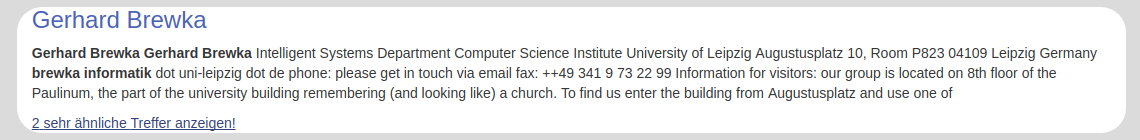
\includegraphics[width=0.99\textwidth]{chapter_data_aqcuisition/grouped_duplicates.png}
	\caption{Ein Dokument mit 2 Fast-Duplikaten}
	\label{fig:grouped_sim}
\end{figure}

\input{chapter_data_aqcuisition/text_profile_algorithm.tex}

Um dies zu ermöglichen, müssen zuerst die (Fast-)Duplikate identifiziert werden.
Dafür wurde das
\href{https://github.com/apache/nutch/blob/master/src/java/org/apache/nutch/crawl/TextProfileSignature.java}{TextProfileSignature}-Verfahren verwendet.
Dieser Algorithmus weist einem Dokument einen Fingerprint zu.
Dabei werden ähnliche Dokumenten auf den gleichen Wert abgebildet.
Algorithmus~\ref{alg:text_profile} zeigt dies im Pseudocode.
In Beispiel~\ref{example:text_profile} wird der Fingerprint für einen Text berechnet.

Nach der Zuweisung des Fingerprints werden entsprechend dem Discovery Scenario alle Paare von Fast-Duplikaten
gesucht~\cite{croft.chap3}. Durch dieses Vorgehen entstehen Gruppen ähnlicher Dokumente.
Für jede solche Gruppe wird ein Repräsentant gewählt\footnote{Das längste Dokument wird der Vertreter.}.
Dieser wird um die URLs der anderen Gruppenmitglieder angereichert.
Abschließend werden die restlichen Dokumente einer Gruppe gelöscht\footnote{Die Implementierung ist in dem Modul 
\href{https://github.com/mam10eks/search-homepage-of-university-leipzig/tree/master/custom-index-cleaning}
{Custom Index Cleaning} zu finden.}.

\newpage
\input{chapter_data_aqcuisition/text_profile_example.tex}


\newpage
\section{Verarbeitung von Anfragen}
\label{chap:query_processing}

Die Verarbeitung von Anfragen\footnote{Auch Query Processing} wird im Allgemeinen durch drei Komponenten realisiert~\cite{croft.chap2}.
Auch die im Rahmen dieser Arbeit erstellte Suchmaschine bildet davon keine Ausnahme.
Dementsprechend werden in den folgenden Abschnitten die Bestandteile User Interaction, Ranking und Evaluation vorgestellt.

\subsection{User Interaction~\cite{croft.chap2}}
\label{chap:user_interaction}

Die Komponente zur Nutzerinteraktion bietet eine Schnittstelle\footnote{Der Quellcode ist in dem Modul
\href{https://github.com/mam10eks/search-homepage-of-university-leipzig/tree/master/search-engine-backend}{search-engine-backend}
enthalten.}
zwischen dem Benutzer und der Suchmaschine.
Um diesem Nutzer eine gewohnte Usability inklusive intuitiver Bedienung zu ermöglichen,
wurden die in der Praxis verbreiteten Standards eingehalten.

\begin{wrapfigure}{H}{0.49\linewidth}
	\vspace*{-0.4cm}
	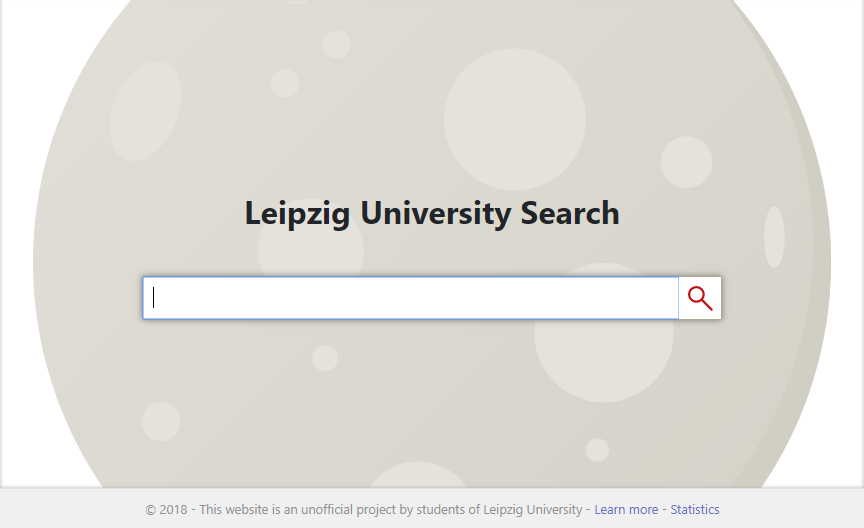
\includegraphics[width=0.48\textwidth]{chapter_query_processing/frontend_landing_page.png}
	\caption{Die Landing Page der Suchmaschine}
	\label{fig:landing_page}
	\vspace*{-0.2cm}
\end{wrapfigure}


Dementsprechend muss einem Nutzer das Absenden von Anfragen ermöglicht werden.
Dafür ist es üblich, eine Landing Page mit prominent mittig platzierter Eingabemaske auszuliefern\cite{baeza_yates.search_interfaces}.
Abbildung~\ref{fig:landing_page} zeigt dies für die im Rahmen dieser Arbeit entwickelte Suchmaschine.

Nachdem ein Nutzer seine Anfrage spezifiziert hat, werden ihm die Ergebnisse präsentiert.
Dafür erhält die Schnittstelle eine für die Query gerankte Liste von Dokumenten von der Ranking-Komponente.
Diesbezüglich ist es gängig, einem Benutzer für kleinere Ausschnitte aus der Dokumentliste jeweils 
ausgewählte Metadaten in Verbindung mit einem 
für die Anfrage besonders relevanten Textausschnitt\footnote{Sogenannte Snippets} zu präsentieren~\cite{baeza_yates.search_interfaces}.
Relevante Wörter werden dabei speziell hervorgehoben.
Die unter Berücksichtigung dieser Punkte entstandene Search Engine Result Page\footnote{SERP} wird in Abbildung~\ref{fig:serp} vorgestellt.

\begin{figure}[!ht]
	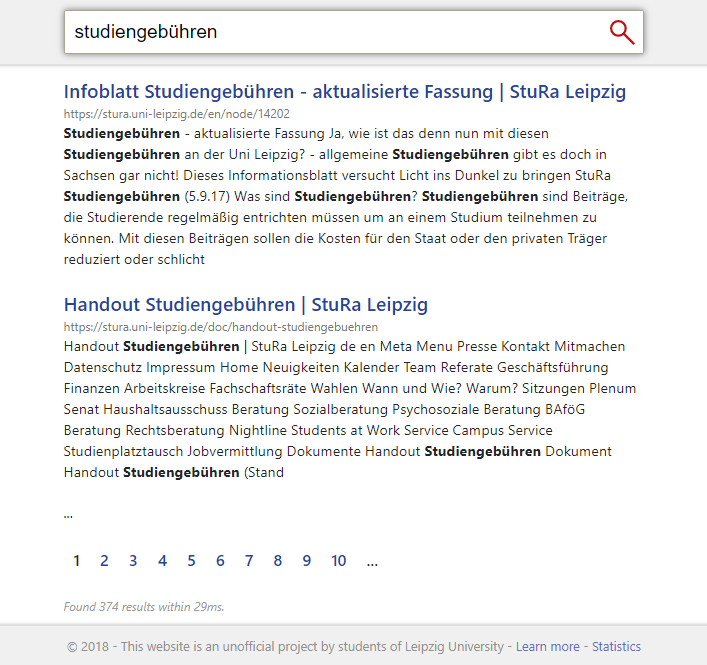
\includegraphics[width=0.99\textwidth]{chapter_query_processing/serp.png}
	\caption{Die SERP für die Anfrage \glqq studiengebühren\grqq}
	\label{fig:serp}
\end{figure}

In der Regel wird einem Nutzer die Formulierung und Spezialisierung seiner Anfragen durch verschiedene Hilfsmittel
erleichtert.
In dem vorliegenden Projekt wurde eine Query Suggestion implementiert,
welche Vervollständigungsvorschläge auf Basis populärer Anfragen liefert.
Die dafür notwendige, dynamische Benutzerschnittstelle wird in Abbildung~\ref{fig:query_suggestions} gezeigt.
Verwandte Maßnahmen zur Verbesserungen der Benutzbarkeit wie Spell Checking oder Query Refinement 
wurden zugunsten anderer Features nicht umgesetzt.

\begin{figure}[!ht]
	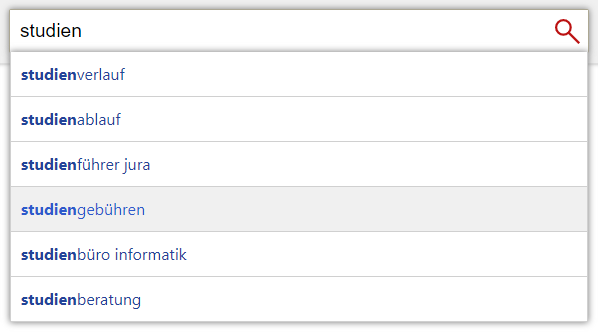
\includegraphics[width=0.99\textwidth]{chapter_query_processing/autocomplete.png}
	\caption{Query Suggestions für die Eingabe: studien}
	\label{fig:query_suggestions}
\end{figure}

Um den Suchmaschinenservice einem möglichst breiten Nutzerkreis zuzuführen, sind die
Komponenten zur Benutzerinteraktion in Form eines Webfrontends realisiert. Für die Entwicklung
werden die jeweils aktuellen Standards HTML5, CSS3 sowie JavaScript eingesetzt. 
Ausgeliefert werden diese Bestandteile durch einen Express-Webserver, welcher im Rahmen einer NodeJS-Anwendung betrieben wird.
Aus Kompatibilitätsgründen werden Teile der Bootstrap-Library eingebunden.
Falls ein Browser die History-API unterstützt, wird diese zur
Bereitstellung von Deep-Links ohne einen Full-Page-Refresh
geeigneter Seiten\footnote{Zum Beispiel die About-Page.} verwendet.

Der Zugriff auf die Ranking-Komponente (siehe Abschnitt~\ref{chap:ranking}) und Query-Suggestions wird durch
entsprechende \href{https://en.wikipedia.org/wiki/Representational_state_transfer}{REST-Endpunkte} ermöglicht.
Bereitgestellt werden diese durch eine \href{https://projects.spring.io/spring-boot/}{Spring-Boot-Anwendung}.
Die Query-Suggestions unterscheiden dabei zwischen nutzerbezogenen und globalen Vorschlägen.
Durch nutzerbezogene Vorschläge ist es einem Nutzer möglich, von ihm bereits getätigte Anfragen zu wiederholen.
Globale Vorschläge identifizieren innerhalb der Suchmaschine populäre Anfragen mit Hilfe von Logdaten.
Für eine sinnvolle initiale Menge von globalen Vorschlägen wurden semantisch passende
Vorschläge von Google gecrawlt und eingepflegt\footnote{Der Quellcode für den Crawler ist TODO link zum Code.
Damit wurden 2639 Vorschläge generiert}.


\subsection{Ranking~\cite{croft.chap2}}
\label{chap:ranking}
\input{chapter_query_processing/ranking.tex}


\subsection{Evaluation~\cite{croft.chap2}}
\label{chap:evaluation}
\input{chapter_query_processing/evaluation.tex}


\newpage
\section{Analyse der Logdaten}
\label{chap:log_analysis}

Bla

\subsection{Durchführung eines Laborexperiments}
\label{chap:labroratory_experiment}

Bla


%************************************************************************************************************************
%* bibliography
%************************************************************************************************************************
\newpage
\addcontentsline{toc}{section}{Literatur}
\bibliography{literature}
\bibliographystyle{alpha}

\end{document}


%************************************************************************************************************************
%* begin document
%************************************************************************************************************************
\begin{document}
\thispagestyle{empty}

\begin{center}
\large

\vspace{1cm}
\textbf{\sffamily	Universität Leipzig\\
			Fakultät für Mathematik und Informatik\\
			Institut für Informatik\\}

\vspace{2cm}
{\Large\textbf{\sffamily Kurs Information Retrieval}}


\large

Praktikumsbericht
\vspace{1cm}
\end{center}

\textbf{Zusammenfassung}:\\
\phantomsection
\label{sec:intro}
Dieser Bericht ...


\vfill

{\large
\begin{tabular}{p{7cm} l}
&\\
\small
Leipzig, März 2018 		& \small vorgelegt von\\
				& \small Maik Fröbe, Danilo Morgado, Sebastian Günther\\
\end{tabular}}

\begin{tabular}{p{7cm} l}
&\\
\small
Betreuer: 	& \small Jun.-Prof. Dr. Martin Potthast \\
				& \small Fakultät für Mathematik und Informatik\\
				& \small Text Mining und Retrieval
\end{tabular}

%************************************************************************************************************************
%* main chapters
%************************************************************************************************************************
\pagenumbering{arabic}

\newpage
\section{Von der Datenbeschaffung zum fertigen Index}
\label{chap:data_aqcuisition}

Die in einer Dokumentensammlung enthaltenen Informationen
tragen fundamental zum Erfolg einer Suchmaschine bei~\cite{croft.chap3}.
Dementsprechend stellt eine geeignete, mit vertretbarem Aufwand durchführbare
Erzeugung dieser Dokumentensammlung den Anfang der Wertschöpfungskette dar.

Die im Kontext von Web-Suchmaschinen dafür benötigten Programme werden Crawler genannt~\cite{croft.chap3}.
Diese beschäftigen sich damit, Webseiten zu finden und herunterzuladen, um sie für spätere Verarbeitungsschritte lokal Verfügbar zu haben.
Die in der \hyperref[sec:intro]{Problembeschreibung} dargestellte Beschränkung auf die Website der Universität Leipzig
vereinfacht dieses, im Allgemeinen sehr anspruchsvolle Problem, und wird als Site Search bezeichnet~\cite{croft.chap2}.

Im Rahmen dieser Arbeit wurde zur Erzeugung der Dokumentensammlung die freie Software~\cite{wiki.free_license}
Apache Nutch\footnote{Nutch ist~\href{https://github.com/apache/nutch/blob/master/LICENSE.txt}{unter Apache Version 2.0 lizensiert}.}
verwendet.
Nutch übernahm dabei sowohl die Aufgaben eines Crawlers\footnote{Der finale Crawling-Durchgang benötigte 14 Tage um 390 000 Dokumente in 50GB zu sammeln.}
als auch die unmittelbar folgenden Schritte bis einschließlich der Indexerzeugung.
Im Folgenden werden verschiedene, während der Arbeit angewandten Anpassungen und Vereinfachungen des von Nutch bereitgestellten
Workflows vorgestellt.
 
\subsection{Domänenspezifische, manuell gepflegte Selectivity}
Unter den Features, die ein Crawler umsetzen sollte~\cite{manning.chap20},
findet sich auch die Notwendigkeit, die Qualität der zu crawlenden Seiten
in die Crawling-Reihenfolge einfließen zu lassen.
Am Beispiel von Nutch ist diese Funktionalität durch eine Bewertung der einzelnen Seiten
auf Basis der aktuell bekannten Linkstruktur realisiert~\cite{nutch.invert_links}.
Dabei werden Seiten, welchen eine höhere Wichtigkeit vorhergesagt wird, zeitiger heruntergeladen.

Aufgrund begrenzter Ressourcen wurde diese Idee weiter verschärft,
so dass bestimmte Seiten erst gar nicht gecrawlt wurden.
Dies betrifft Seiten, welche nicht direkt zur Universität gehören,
sowie Spider-Traps\footnote{Zum Beispiel ein
\href{http://www.informatik.uni-leipzig.de/~meyer/?d=15}{Kalender mit dynamisch erzeugten Links}.},
umfangreiche Webanwendungen\footnote{Zum Beispiel die 
\href{http://wortschatz.uni-leipzig.de/de}{Wortschatz}-, verschiedene 
\href{http://www.informatik.uni-leipzig.de/~duc/TD/td/index.php?bpos=72&db=ev}{Wörterbuch}-, oder auch
\href{http://pcai003.informatik.uni-leipzig.de/kosemnet/}{Semantic-Web}-Anwendungen.},
oder auch vollständige Suchmaschinen\footnote{Zum Beispiel ein
\href{http://lips.informatik.uni-leipzig.de/}{Dokumentenserver für Abschlussarbeiten}.} innerhalb der Universität.

Insbesondere für die Letzteren besteht die Herausforderung darin,
genug Informationen über Existenz und Einsatzzweck einer solchen Seite zu sammeln,
ohne gleichzeitig unnötig vielen dynamisch erzeugten Links zu folgen.
Beispiel~\ref{example:document_server} beschreibt dies am Fall eines Dokumentenservers.

\begin{example}[Dokumentenserver FMI]{example:document_server}
	Der \href{http://lips.informatik.uni-leipzig.de/}{Dokumentenserver der Fakultät für Mathematik und Informatik}
	stellt unter anderem folgende Funktionalitäten bereit:

	\textbf{Den Download von Dokumenten:}\\
	Ein Nutzer kann die im Dokumentenserver enthaltenen Dokumente herunterladen.
	Dazu besitzt jedes Dokument eine Übersichtsseite, welche Metadaten zum Dokument bereitstellt sowie
	einen Link zum vollständigen Dokument.
	Beispiele dafür sind:
	\begin{itemize}
		\item Eine Übersichtsseite: \url{http://lips.informatik.uni-leipzig.de/pub/2017-0}
		\item Ein Dokument: \url{http://lips.informatik.uni-leipzig.de/files/thesis.pdf}
	\end{itemize}
	Beide enthalten wichtige Informationen und sollten gecrawlt werden.

	\textbf{Das Filtern nach Dokumenten:}\\
	Ein Nutzer kann über eine Facettensuche~\cite{wiki.facetted_search} innerhalb der Dokumente filtern.
	Beispiele dafür sind:
	\begin{itemize}
		\item Filterung nach \glqq Organisation IfI\grqq: \url{http://lips.informatik.uni-leipzig.de/browse/results/taxonomy%3A912}
		\item Filterung nach \glqq Organisation IfI und Author Erhard Rahm\grqq:\\ \url{http://lips.informatik.uni-leipzig.de/browse/results/taxonomy%3A912%20field_authors%3A%22Rahm%2C%20Erhard%22}
	\end{itemize}
	Die enorme Menge an möglichen Filter-Permutationen,
	sowie \href{http://se-pubs.dbs.uni-leipzig.de/pubs/results/0%200%200%200%20taxonomy%3A30%2C696}
		{teilweise auftretenden Endlosschleifen} lassen den Aufwand für ein Crawling dieser Seiten als unangemessen erscheinen.
	Dies wird abgerundet durch den Umstand, dass die oben beschriebenen Zielseiten ohne Filterung erreichbar sind.
	Dazu ist eine Traversierung von folgenden Seiten sinnvoll:
	\begin{itemize}
		\item Die erste Seite einer Liste aller vorhandenen Dokumente: \url{http://lips.informatik.uni-leipzig.de/browse/results/}
		\item Für welche nachfolgende Seiten direkt über Links zugänglich sind:
		\url{http://lips.informatik.uni-leipzig.de/browse/results?page=4}
	\end{itemize}
\end{example}


Um derartige Problemfälle zu behandeln müssen diese im ersten Schritt identifiziert werden.
Diesbezüglich bietet es sich an, während kleinerer Probe-Crawlings eine Auswertung der Logs vorzunehmen.
Um dies in vereinfachter Form durchzuführen,
wurde ein Statistik-Plugin für Nutch implementiert\footnote{Das Statistik-Plugin kann in dem
\href{https://github.com/DaniloMorgado/url_statistic_plugin}{entsprechenden Github-Repository} eingesehen werden.}.
Dieses Plugin identifiziert mittels
Map-Reduce\footnote{Einführungen in das Map-Reduce-Paradigma können hier eingesehen werden: \cite{wiki.mapreduce},
\cite{nosql.mapreduce}, \cite{hadoop.mapreduce}.}
Bereiche für die der Crawler besonders aktiv wird.
Dazu werden alle bekannten URLs durch Entfernung
von Queries oder Fragmenten normalisiert, und in ihre hierarchischen Bestandteile zerlegt.
Beispiel~\ref{example:statistic_plugin} zeigt dies für eine Auswahl der in
Beispiel~\ref{example:document_server} besprochenen Links,
wie durch Aufsummieren dieser Bestandteile die Ausgabe des Plugins erzeugt wird.

\begin{example}[Berechnungsschritte des Statistik-Plugins]{example:statistic_plugin}
Die Map-Phase nimmt die Normalisierung der Links, sowie eine Umwandlung in die hierarchischen Bestandteile vor:\\

http://lips.informatik.uni-leipzig.de/pub/2017-0\\
$\rightarrow$ \\
$[$(http://lips.informatik.uni-leipzig.de, 1),\\
(http://lips.informatik.uni-leipzig.de/pub, 1),\\
(http://lips.informatik.uni-leipzig.de/pub/2017-0, 1)$]$\\

http://lips.informatik.uni-leipzig.de/files/thesis.pdf\\
$\rightarrow$\\
$[$
(http://lips.informatik.uni-leipzig.de, 1), \\
(http://lips.informatik.uni-leipzig.de/files, 1), \\
(http://lips.informatik.uni-leipzig.de/files/thesis.pdf, 1)
$]$\\

Die Reduce Phase summiert alle eintreffenden Paare bestehend aus Link-Bestandteil und count:\\

$[$
(http://lips.informatik.uni-leipzig.de, 2), \\
(http://lips.informatik.uni-leipzig.de/pub, 1), \\
...
$]$
\end{example}


In der Ausgabe des Statistik-Plugins können schließlich sinnvoll Problemfälle identifiziert
werden\footnote{Neben den in Beispiel~\ref{example:document_server} hervorgehobenen Problemen sei hier noch auf potentiell fehlende Seiten hingewießen.
Diese können durch einen Vergleich der aufsummierten Linkbestandteile mit der Anzahl der von Google indexierten Seiten entdeckt werden.}.
Um dies effizient durchführen zu können,
bietet es sich an, dieses Plugin als Eingabe für existierende Standardwerkzeuge zu nutzen.
So erlaubt die nach Anzahl sortierte sowie durch einen Mindest-Threshold und White-List gefilterte Ausgabe
auf den ersten Blick potentielle Probleme zu identifizieren.

Im nächsten Schritt ist es notwendig, diese Problemfälle zu behandeln.
Eine einfache, aber effiziente Möglichkeit, dies umzusetzen, wird in Nutch in Form von \href{https://github.com/apache/nutch/blob/master/conf/regex-urlfilter.txt.template}{Regex-URL-Filtern} bereitgestellt.
Darunter versteht man eine Liste von requlären Ausdrücken, welche jeweils um eine positive oder negative Markierung erweitert sind.
Für eine URL werden die regulären Ausdrücke dann der Reihe nach ausgewertet.
Der erste passende Ausdruck entscheidet, ob eine URL gecrawlt werden darf (falls der zugehörige Ausdruck positiv markiert ist),
oder nicht\footnote{Aus diesem Grund ist es üblich, 
die Liste der Ausdrücke mit einem entsprechendem immer zutreffendem Eintrag abzuschließen.}.

Die in Nutch vordefinierten Regex-URL-Filter verfolgen das Ziel,
das Crawling auf sinnvolle Protokolle\footnote{HTTP, kein mailto- oder file-Protokoll.}
und Dokumenttypen\footnote{HTML-Seiten, keine CSS-Resourcen, Bilder oder Videos.} zu beschränken.
Um diese Filter systematisch korrekt zu erweitern wurde ein
testgetriebenes Vorgehen gewählt\footnote{Die Implementierung befindet
sich in dem Github-Repository \href{https://github.com/mam10eks/check-nutch-regex-urlfilter}{check-nutch-regex-urlfilter}.}.
Dieses zeichnet sich durch die Möglichkeit aus, einzelne Bereiche getrennt voneinander zu konfigurieren, ohne ungewünschte Seiteneffekte zu erzeugen.

Nach dem \href{https://de.wikipedia.org/wiki/Teile-und-herrsche-Verfahren}{Teile-und-herrsche-Verfahren} werden
diesbezüglich für kleine Bereiche der zu crawlenden Webseiten einzeln anhand von Beispielen Konfigurationen vorgenommen.
Dafür werden für diesen Bereich Positiv- und Negativ-Beispiele in Form von URLs zusammengetragen.
Im nächsten Schritt werden die für diese Beispiele passenden Regex-URL-Regeln aufgestellt.
Diese verfolgen das Ziel, dass sie sich für alle Positivbeispiele zu positiv auswerten, und für alle Negativbeispiele entsprechend zu negativ.
Beispiel~\ref{example:regex_url} verdeutlicht dies für die aus Beispiel~\ref{example:document_server} bekannten URLs.

Die Konfigurationen der einzelnen Bereiche werden schließlich \href{https://de.wikipedia.org/wiki/Top-down_und_Bottom-up}{Bottom-up} zu einer einzigen 
URL-Filter-Liste vereinigt.
Für diese Liste werden anschließend alle Positiv- und Negativ-Beispiele evaluiert.
Nur wenn dabei für alle Beispiele das spezifizierte Verhalten beobachtet wird, ist diese URL-Liste valide und kann verwendet werden.

\begin{example}[Erstellung der Regex-URL-Regeln für den Dokumentenserver]{example:regex_url}
\# Positivbeispiele: Stelle sicher, dass die Dokumente gecrawlt werden\\
http://lips.informatik.uni-leipzig.de/browse/results?page=4\\
http://lips.informatik.uni-leipzig.de/files/thesis.pdf\\
http://lips.informatik.uni-leipzig.de/pub/2017-0

\# Negativbeispiele: Verhindere, dass die Filterfunktion genutzt wird\\
http://lips.informatik.uni-leipzig.de/browse/results/taxonomy%3A912

\# Regex-URL-Regeln, welche diese Anforderungen erfüllen\\
+http://lips.informatik.uni-leipzig.de/(pub|files)/.*\\
+http://lips.informatik.uni-leipzig.de/browse/results.*\\
-http://lips.informatik.uni-leipzig.de.*\\
\end{example}


Durch diese Hilfswerkzeuge wurde im Rahmen der Arbeit die Website der Universität Leipzig anhand ihrer Fakultäten auf die einzelnen Bearbeiter aufgeteilt.
Mit einer Reihe von Probe-Crawlings konnte die vollständige Regex-URL-Filter-Liste erstellt werden.
Diese Vorbereitung unterstützte das unterbrechungsfreie Crawling der für den Index verwendeten Dokumente.
Dafür konnten die entstandenen Positivbeispiele direkt als \href{https://wiki.apache.org/nutch/NutchTutorial#Create_a_URL_seed_list-1}{Seeds} eingesetzt werden.

\subsection{Reproduzierbare Erzeugung eines Lucene Index mit Docker und Solr}

Um die gecrawlten Dokumente in der in Abschnitt~\ref{chap:ranking} beschriebenen Suchmaschine verfügbar zu machen, müssen sie in einen Lucene Index überführt werden.

Dafür wird im ersten Schritt eine sogenannte Conversion durchgeführt~\cite{croft.chap2}.
Dabei werden im vorliegenden Fall gecrawlte Dokumente,
welche in den unterschiedlichsten Formaten vorliegen können\footnote{Häufigstes Format war HTML, aber auch PDF, Word oder Power Point waren vertreten.}
in ein einheitliches Format umgewandelt.
Auf eine mögliche Reduzierung der Dokumente auf deren Main-Content wurde
verzichtet\footnote{Die Extraktion des Main-Content ist mit Apache Tika
unmittelbar möglich. Jedoch erschien es plausibel, dass für die gecrawlten Webseiten mit vergleichsweiße wenig Rauschen zu rechnen ist.}.
Realisiert wurde die Conversion mit \href{https://en.wikipedia.org/wiki/Apache_Tika}{Apache Tika}.

Anschließend wird mit Nutch eine \href{https://wiki.apache.org/nutch/bin/nutch_invertlinks}{Inversion der Links} durchgeführt.
Dabei werden für alle Dokumente die Texte der eingehenden Links in dedizierten Feldern an dem Dokument abgespeichert.
Im nächsten Schritt wird eine \href{https://github.com/apache/nutch/blob/master/src/java/org/apache/nutch/crawl/TextProfileSignature.java}{Near Duplicate Detection}
durchgeführt, welche näher in Abschnitt~\ref{chap:near_duplicate_detection} erläutert wird.

Nutch kann den Lucene Index nicht selbstständig erzeugen.
Aus diesem Grund wird mit einem \href{http://lucene.apache.org/solr/}{Solr Server} ein Index über die gecrawlten Dokumente erzeugt.
Diesbezüglich wird mit Solr eine Text Transformation~\cite{croft.chap2} durchgeführt.
Dabei wurde entsprechend der Standards auf eine Entfernung von Stoppwörtern sowie Stemming
verzichtet\footnote{Jedoch gehört das testen unterschiedlicher 
\href{https://github.com/apache/lucene-solr/blob/master/lucene/analysis/common/src/java/org/apache/lucene/analysis/core/StopFilterFactory.java}{Stoppwortlisten} sowie verschiedener
\href{https://github.com/apache/lucene-solr/blob/master/lucene/analysis/common/src/java/org/apache/lucene/analysis/en/PorterStemFilterFactory.java}{Stemmer}
zu dem geplanten Vorgehen,
die Effektivität der Suchmaschine für das durchgeführte Laborexperiment zu optimieren (Siehe Kapitel~\ref{chap:log_analysis}).}.
Die eigentliche Indexerzeugung mit Solr schließt diesen Prozess ab.
Dabei werden neben den Dokument-Statistiken~\cite{croft.chap2} für das spätere Scoring von Dokumenten auch Vorbereitungen zur Erzeugung von Snippets vorgenommen.
Der so erzeugte Index kann unmittelbar in Lucene eingesetzt werden.

Die hier beschriebene Erzeugung des Index aus den gecrawlten Dokumenten ist von vielen Parametern abhängig.
Dadurch wird eine häufige Wiederholung dieses Prozesses sinnvoll, um die Auswirkung von Anpassungen an verschiedenen Parametern zu prüfen.
Um den Aufwand dafür gering zu halten, wurde der komplette Workflow reproduzierbar automatisiert\footnote{Das
entsprechende Github-Repository mit
den Scripten und der Konfiguration ist \href{https://github.com/mam10eks/nutch_tools/}{Nutch-Tools}.}.

Dafür wird als Eingabe eine Menge von Nutch-Crawl-Directories erwartet.
Diese werden im ersten Schritt bereinigt, um ein erneutes Parsing der rohen Dokumente durchzuführen.
Danach werden die einzelnen, oben beschriebenen Arbeitsschritte durchgeführt.
Sobald die Indexerzeugung beginnt, wird der dafür notwendige Solr-Server mit Docker
bereitgestellt. Da die notwendige Konfiguration sowie das Index-Schema in den Container gemountet werden,
ist auch dieser Schritt einfach wiederholbar.

\subsection{Data Cleaning: Aggregation von Fast-Duplikaten}
\label{chap:near_duplicate_detection}

Duplikate und Fast-Duplikate treten in vielen Situationen auf~\cite{croft.chap3}.
Im Rahmen dieser Arbeit war die entsprechende Zielsetzung, diese transparent an den Nutzer zu kommunizieren.
Abbildung~\ref{fig:grouped_sim} stellt dies an einem Beispiel dar.

\begin{figure}[!ht]
	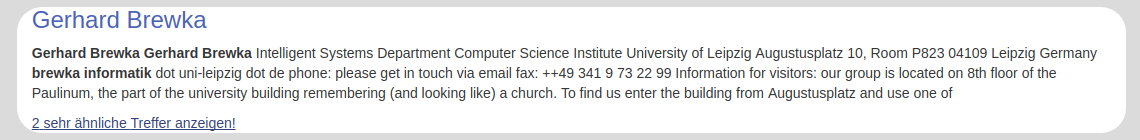
\includegraphics[width=0.99\textwidth]{chapter_data_aqcuisition/grouped_duplicates.png}
	\caption{Ein Dokument mit 2 Fast-Duplikaten}
	\label{fig:grouped_sim}
\end{figure}

\begin{wrapfigure}{H}{0.51\linewidth}
	\vspace*{-0.4cm}

\begin{scriptsize}
\begin{algorithm}[H]
	\SetKwInOut{Input}{Input}
	\SetKwInOut{Output}{Output}
		       
	\Input{ Document $\mathcal{D}$, $min$ $\in$ $\mathbb{N}^{+}$, $\mathcal{Q}$ $\in$ $\mathbb{R}$}
	\Output{ Fingerprint for Document $\mathcal{D}$}

	$\mathcal{D}$ $\gets$ removeNonAlphanumericCharacters($\mathcal{D}$)\\
	$\mathcal{D}$ $\gets$ toLowerCase($\mathcal{D}$)\\
	$\mathcal{T}$ $\gets$ tokenizeWithFrequencyCount($\mathcal{D}$)\\
	$\mathcal{T}$ $\gets$ removeTokensShorterOrEqualThan($min$, $\mathcal{T}$)\\
	$\mathcal{T}$ $\gets$ roundFreqeunciesDownToNearestMultiple($\mathcal{Q}$, $\mathcal{T}$)\\
	$\mathcal{T}$ $\gets$ removeTokensWithTooSmallFrequency($\mathcal{Q}$, $\mathcal{T}$)\\

	return md5Hash(sort($\mathcal{T}$))\\
	\caption{Text Profile}
	\label{alg:text_profile}
\end{algorithm}
\end{scriptsize}

	\vspace*{-0.2cm}
\end{wrapfigure}


Um dies zu ermöglichen, müssen zuerst die (Fast-)Duplikate identifiziert werden.
Dafür wurde das
\href{https://github.com/apache/nutch/blob/master/src/java/org/apache/nutch/crawl/TextProfileSignature.java}{TextProfileSignature}-Verfahren verwendet.
Dieser Algorithmus weist einem Dokument einen Fingerprint zu.
Dabei werden ähnliche Dokumenten auf den gleichen Wert abgebildet.
Algorithmus~\ref{alg:text_profile} zeigt dies im Pseudocode.
In Beispiel~\ref{example:text_profile} wird der Fingerprint für einen Text berechnet.

Nach der Zuweisung des Fingerprints werden entsprechend dem Discovery Scenario alle Paare von Fast-Duplikaten
gesucht~\cite{croft.chap3}. Durch dieses Vorgehen entstehen Gruppen ähnlicher Dokumente.
Für jede solche Gruppe wird ein Repräsentant gewählt\footnote{Das längste Dokument wird der Vertreter.}.
Dieser wird um die URLs der anderen Gruppenmitglieder angereichert.
Abschließend werden die restlichen Dokumente einer Gruppe gelöscht\footnote{Die Implementierung ist in dem Modul 
\href{https://github.com/mam10eks/search-homepage-of-university-leipzig/tree/master/custom-index-cleaning}
{Custom Index Cleaning} zu finden.}.

\newpage
\begin{example}[Berechnung des Fingerprints mittels TextProfileSignature]{example:text_profile}
	\textbf{Eingabe:}\\
		$\mathcal{D}$ $=$ \glqq Tropical fish include fish found in tropical environments around the world,
			including both freshwater and salt water species.\grqq,
		MINLENGTH $=$ $2$, QuantRate $=$ $0.01$\\
	
	\textbf{Tokenisierung und Filterung nach Wortlänge:}\\
		$\{$ (include, 1), (including, 1), (salt, 1), (environments, 1), (around, 1), (water, 1),
			(both, 1), (tropical, 2), (the, 1), (found, 1), (world, 1), (species, 1), (and, 1), (fish, 2), (freshwater, 1) $\}$\\

	\textbf{Filtere Einträge, deren Quantity unter Threshold liegt:}\\
		textProfile $=$ $\{$ (tropical, 2), (fish, 2) $\}$\\
	
	\textbf{Berechne Signatur:}\\
		sort(textProfile)\\
		textProfileSignature $=$ md5Hash(textProfile)
\end{example}



\newpage
\section{Verarbeitung von Anfragen}
\label{chap:query_processing}

Die Verarbeitung von Anfragen\footnote{Auch Query Processing} wird im Allgemeinen durch drei Komponenten realisiert~\cite{croft.chap2}.
Auch die im Rahmen dieser Arbeit erstellte Suchmaschine bildet davon keine Ausnahme.
Dementsprechend werden in den folgenden Abschnitten die Bestandteile User Interaction, Ranking und Evaluation vorgestellt.

\subsection{User Interaction~\cite{croft.chap2}}
\label{chap:user_interaction}

Die Komponente zur Nutzerinteraktion bietet eine Schnittstelle\footnote{Der Quellcode ist in dem Modul
\href{https://github.com/mam10eks/search-homepage-of-university-leipzig/tree/master/search-engine-backend}{search-engine-backend}
enthalten.}
zwischen dem Benutzer und der Suchmaschine.
Um diesem Nutzer eine gewohnte Usability inklusive intuitiver Bedienung zu ermöglichen,
wurden die in der Praxis verbreiteten Standards eingehalten.

\begin{wrapfigure}{H}{0.49\linewidth}
	\vspace*{-0.4cm}
	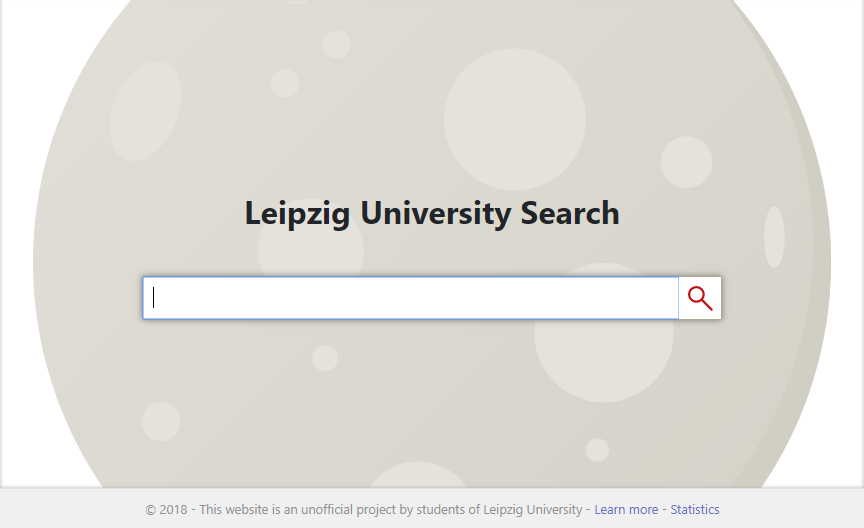
\includegraphics[width=0.48\textwidth]{chapter_query_processing/frontend_landing_page.png}
	\caption{Die Landing Page der Suchmaschine}
	\label{fig:landing_page}
	\vspace*{-0.2cm}
\end{wrapfigure}


Dementsprechend muss einem Nutzer das Absenden von Anfragen ermöglicht werden.
Dafür ist es üblich, eine Landing Page mit prominent mittig platzierter Eingabemaske auszuliefern\cite{baeza_yates.search_interfaces}.
Abbildung~\ref{fig:landing_page} zeigt dies für die im Rahmen dieser Arbeit entwickelte Suchmaschine.

Nachdem ein Nutzer seine Anfrage spezifiziert hat, werden ihm die Ergebnisse präsentiert.
Dafür erhält die Schnittstelle eine für die Query gerankte Liste von Dokumenten von der Ranking-Komponente.
Diesbezüglich ist es gängig, einem Benutzer für kleinere Ausschnitte aus der Dokumentliste jeweils 
ausgewählte Metadaten in Verbindung mit einem 
für die Anfrage besonders relevanten Textausschnitt\footnote{Sogenannte Snippets} zu präsentieren~\cite{baeza_yates.search_interfaces}.
Relevante Wörter werden dabei speziell hervorgehoben.
Die unter Berücksichtigung dieser Punkte entstandene Search Engine Result Page\footnote{SERP} wird in Abbildung~\ref{fig:serp} vorgestellt.

\begin{figure}[!ht]
	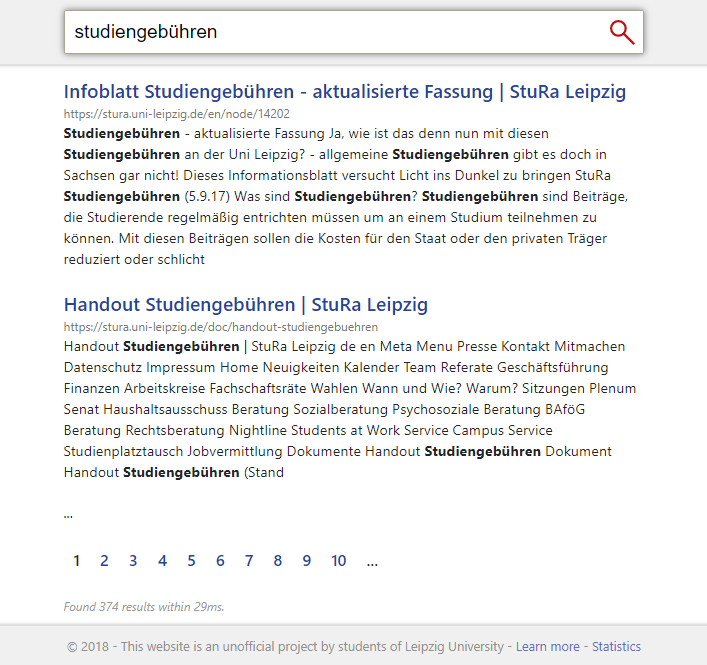
\includegraphics[width=0.99\textwidth]{chapter_query_processing/serp.png}
	\caption{Die SERP für die Anfrage \glqq studiengebühren\grqq}
	\label{fig:serp}
\end{figure}

In der Regel wird einem Nutzer die Formulierung und Spezialisierung seiner Anfragen durch verschiedene Hilfsmittel
erleichtert.
In dem vorliegenden Projekt wurde eine Query Suggestion implementiert,
welche Vervollständigungsvorschläge auf Basis populärer Anfragen liefert.
Die dafür notwendige, dynamische Benutzerschnittstelle wird in Abbildung~\ref{fig:query_suggestions} gezeigt.
Verwandte Maßnahmen zur Verbesserungen der Benutzbarkeit wie Spell Checking oder Query Refinement 
wurden zugunsten anderer Features nicht umgesetzt.

\begin{figure}[!ht]
	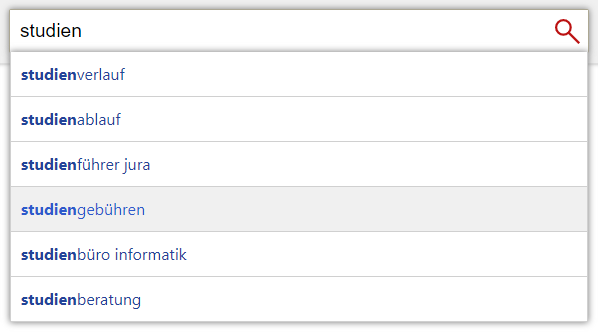
\includegraphics[width=0.99\textwidth]{chapter_query_processing/autocomplete.png}
	\caption{Query Suggestions für die Eingabe: studien}
	\label{fig:query_suggestions}
\end{figure}

Um den Suchmaschinenservice einem möglichst breiten Nutzerkreis zuzuführen, sind die
Komponenten zur Benutzerinteraktion in Form eines Webfrontends realisiert. Für die Entwicklung
werden die jeweils aktuellen Standards HTML5, CSS3 sowie JavaScript eingesetzt. 
Ausgeliefert werden diese Bestandteile durch einen Express-Webserver, welcher im Rahmen einer NodeJS-Anwendung betrieben wird.
Aus Kompatibilitätsgründen werden Teile der Bootstrap-Library eingebunden.
Falls ein Browser die History-API unterstützt, wird diese zur
Bereitstellung von Deep-Links ohne einen Full-Page-Refresh
geeigneter Seiten\footnote{Zum Beispiel die About-Page.} verwendet.

Der Zugriff auf die Ranking-Komponente (siehe Abschnitt~\ref{chap:ranking}) und Query-Suggestions wird durch
entsprechende \href{https://en.wikipedia.org/wiki/Representational_state_transfer}{REST-Endpunkte} ermöglicht.
Bereitgestellt werden diese durch eine \href{https://projects.spring.io/spring-boot/}{Spring-Boot-Anwendung}.
Die Query-Suggestions unterscheiden dabei zwischen nutzerbezogenen und globalen Vorschlägen.
Durch nutzerbezogene Vorschläge ist es einem Nutzer möglich, von ihm bereits getätigte Anfragen zu wiederholen.
Globale Vorschläge identifizieren innerhalb der Suchmaschine populäre Anfragen mit Hilfe von Logdaten.
Für eine sinnvolle initiale Menge von globalen Vorschlägen wurden semantisch passende
Vorschläge von Google gecrawlt und eingepflegt\footnote{Der Quellcode für den Crawler ist TODO link zum Code.
Damit wurden 2639 Vorschläge generiert}.


\subsection{Ranking~\cite{croft.chap2}}
\label{chap:ranking}
Die Ranking-Komponente ist der Kern jeder Suchmaschine.
Sie erzeugt für eine Query aus der User-Interaction-Komponente eine gerankte Liste von Dokumenten.

Dabei beeinflussen deren Effizienz\footnote{Die Verarbeitung vieler Anfragen in kurzer Zeit.}
und Effektivität\footnote{Die Qualität des Rankings: Kann die Suchmaschine relevante Informationen finden?}
die Nützlichkeit der Suchmaschine wesentlich.
Um für beide Anforderungen einen sinnvollen Ausgangspunkt zu schaffen, wurde für das Ranking
\href{https://lucene.apache.org/}{Lucene} verwendet.
Diese Software stellt einen geeigneten Einstieg dar, da darauf andere,
in dieser Domäne verbreitete Softwarekomponenten aufbauen\footnote{Insbesondere die verbreiteten Tools~\cite{dbengines}
\href{https://de.wikipedia.org/wiki/Elasticsearch}{Elasticsearch} und \href{http://lucene.apache.org/solr/}{Solr}
basieren auf Lucene. Deren erweiterter Funktionsumfang, wie Beispielsweiße eine
\href{http://www.searchdatacenter.de/definition/Horizontale-Skalierung-Scale-out}{horizontale Skalierung}, wurde im Rahmen dieser Arbeit nicht benötigt.}.
Verschiedene \href{https://en.wikipedia.org/wiki/Ranking_(information_retrieval)}{Ranking-Algorithmen}
\footnote{Und damit auch 
\href{https://de.wikipedia.org/wiki/Information_Retrieval\#Retrievalmodelle}{Retrieval-Modelle}}
sind in Lucene verfügbar.

Davon wurde \href{https://en.wikipedia.org/wiki/Okapi_BM25}{BM25F} eingesetzt,
da es als Baseline für modernere Ranking-Algorithmen fungiert und für allgemeine
Dokumentsammlungen bessere Ergebnisse\footnote{Entsprechendes Tuning der von BM25F verwendeten Parameter vorrausgesetzt~\cite{baeza_yates.107}.}
erzielt als die verfügbaren,
\href{https://opensourceconnections.com/blog/2015/10/16/bm25-the-next-generation-of-lucene-relevation/}{klassischen Vektor-Modelle}~\cite{baeza_yates.107}.
Dieses \href{https://de.wikipedia.org/wiki/Information_Retrieval#Retrievalmodelle}{Retrieval-Modell}
besitzt die Fähigkeit, mehrere Felder\footnote{Felder werden auch als Attribute oder Features bezeichnet.} in die Berechnung des Scores einfließen zu lassen.
Entsprechend wurden alle verfügbaren Felder 
einbezogen\footnote{Alle Felder mit unmittelbarem Bezug zu dem Inhalt der Dokumente.
Dies sind der vollständige Text eines Dokuments, sowie deren Titel, URL und Anchor-Texte eingehender Links.}.
Da eine sinnvolle Wahl der Attribute\footnote{Einschließlich eventuell abgeleiteter Features.}
und deren Gewichtung im Allgemeinen in
Verbindung mit der User-Relevanz steht, wurden alle Parameter bei ihren Standards belassen.

Das entsprechende Vorgehen für ein Tuning basierend auf Nutzer-Feedback
wird in Abschnitt~\ref{chap:log_analysis} vorgestellt.



\subsection{Evaluation~\cite{croft.chap2}}
\label{chap:evaluation}
Die Aufgabe der Evaluationskomponente ist es, Effizienz und Effektivität zu monitoren.
Dafür muss eine Aufzeichnung des Nutzerverhaltens sowie ausgewählter Systemmetriken vorgenommen werden.

Insbesondere zur Aufzeichnung des Nutzerverhaltens ist eine Identifikation der Nutzer notwendig.
Darauf aufbauend kann protokolliert werden, welcher Nutzer welche Anfragen ausgeführt
hat, welche Ergebnisseiten oder Query-Suggestions einem Nutzer präsentiert wurden,
sowie gegebenenfalls welche Ergebnisse oder Query Suggestions ausgewählt
wurden\footnote{Das erweitern dieser Informationen um die entsprechenden Event-Zeitpunkte erlaubt eine
sinnvolle Rekonstruktion des Nutzerverhaltens.}.

Bei einer technischen Realisierung dieser Punkte fällt auf,
dass es sich um sogenannte \href{https://de.wikipedia.org/wiki/Cross-Cutting_Concern}{Cross-Cutting Concerns}
handelt. Ein bewährtes Mittel derartige Funktionalitäten zu realisieren, ohne die
Komplexität der betroffenen Systemteile unnötig zu ehöhen,
stellt die Aspektorientierte Programmierung\footnote{AOP} dar\cite{spring.chap1.1}.
Die darin verwendeten Aspekte definieren,
was\footnote{In der zugehörigen AOP Terminologie definiert der zu einem Aspekt gehörende Advice die Aufgabe,
also was von dem Aspekt zu erledigen ist~\cite{spring.chap4.1}.}, wann\footnote{Der Advice eines Aspekts definiert 
neben dem was auch zu welchen Zeitpunkten ein Aspekt auszuführen ist.
Unter anderem kann vor, nach, oder das wrappen einer Zielmethode spezifiziert werden\cite{spring.chap4.1}.}
und wo\footnote{Durch sogenannte Pointcuts werden eine oder mehrere Methoden definiert,
an die der Advice gewoben wird\cite{spring.chap4.1}.} auszuführen ist\cite{spring.chap4.1}.

In dem für die Interaction-Komponente verwendeten Framework werden alle Endpunkte über speziell anotierte Methoden
bereitgestellt.
Diesen ist gemein, dass sie ein
\href{https://de.wikipedia.org/wiki/Plain_Old_Java_Object}{POJO}\footnote{Diese sind 
entsprechend einer gewählten Konvention in dem 
\href{https://github.com/mam10eks/search-homepage-of-university-leipzig/tree/master/search-engine-backend}{Backend-Modul}
in zugehörigen \href{https://de.wikipedia.org/wiki/Transferobjekt}{dto} Paketen definiert.}
als Model für die Antwort zurückgeben. 
Dieses Modell wird je nach Endpunkt später in ein HTML-Template\footnote{Spezifiziert innerhalb des 
\href{https://github.com/mam10eks/search-homepage-of-university-leipzig/tree/master/search-engine-backend/src/main/resources/templates}
{templates-Ordner in dem Backend-Modul}.} gerendert oder
JSON-serialisiert.

Unter diesen Vorraussetzungen eignen sich diese Methoden hervorragend,
um sie durch Aspekte um die gewünschten Funktionalitäten zu erweitern\footnote{Schließlich lassen
sie sich eindeutig und generisch über die notwendigen Endpunkt-Anotationen
identifizieren.}.
Dazu wird ein Effizienz-, ein User-Identification-, sowie ein Logging-Aspekt eingesetzt.
Der Effizienz-Aspekt misst dabei Beispielhaft für weitere Systemmetriken die Bearbeitungszeit von Anfragen,
und erweitert das zurückgegebene Model entsprechend.
Der User-Identification-Aspekt stellt
vor dem Aufruf jeder Endpunkt-Methode sicher, dass der Request mit einer
eindeutigen Identifikation des Nutzers versehen ist.
Dies wird über einen Cookie realisiert.
Der Logging-Aspekt protokolliert ausnahmslos alle verfügbaren Informationen.
Dazu notiert er für jeden Endpunkt den Request des Clients zusammen mit dem zurückzugebenden
POJO-Model\footnote{Mit diesem Vorgehen lassen sich alle angesprochenen Informationen zur Rekonstruktion des Nutzer-Verhaltens erheben,
da insbesondere die Links zu den Dokumenten auf dem Server durch Weiterleitungen aufgelöst werden.}.

Die vom Logging-Aspekt protokollierten Informationen können sowohl
Online\footnote{Beispielhaft wurde das im Rahmen dieser Arbeit für die Query-Suggestions vorgenommen.},
als auch Offline analysiert werden.
Um beides zu ermöglichen, wurde mit \href{https://kafka.apache.org/}{Apache Kafka}
eine Streaming Platform mit der Möglichkeit zur persistenten Datenhaltung~\cite{kafka.foreword} eingesetzt.
Dazu publisht der Logging-Aspekt seine Daten als Events nach Kafka.
Um diesen Logging-Aspekt so einfach wie möglich zu halten, bereitet ein
\href{https://www.confluent.io/blog/introducing-kafka-streams-stream-processing-made-simple/}{Stream Processor}
diese Daten weiter auf\footnote{Dieser Stream Processor reichert die Events an und leitet sie
auf sinnvolle Topics um. Der Quellcode ist in dem Modul 
\href{https://github.com/mam10eks/search-homepage-of-university-leipzig/tree/master/search-engine-kafka-streams}
{search-engine-kafka-streams} enthalten.}.
Online-Analysen wie die Query-Suggestion können sich nun unmittelbar an die für sie interessanten Events subscriben.
Offline Analysen können die persistierten Events gleichzeitig in einem  Batch-Vorgang verarbeiten.
Als Beispiel dafür stellt Abbildung~\ref{fig:visualization} einen mit Python realisierten
Import\footnote{Der Quellcode ist in dem Modul
\href{https://github.com/mam10eks/search-homepage-of-university-leipzig/tree/master/visualize_events}{visualize\_events}.}
der Events nach \href{https://de.wikipedia.org/wiki/Neo4j}{Neo4j} zur Visualisierung dar.

\begin{figure}[!ht]
	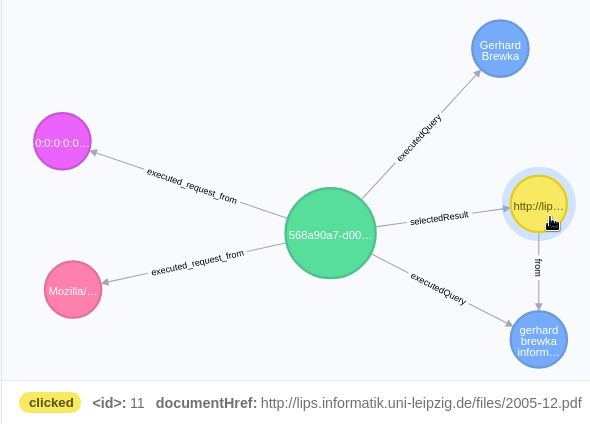
\includegraphics[width=0.99\textwidth]{chapter_query_processing/example_neo4j_visualization.png}
	\caption{Beispielgraph im
	\href{https://neo4j.com/developer/guide-neo4j-browser/}{Neo4j-Browser}
	einer User-Session bestehend aus 2 Anfragen, bei denen bei einer Anfrage ein Ergebniss angeklickt wurde.}
	\label{fig:visualization}
\end{figure}

Die hier vorgestellte Evaluationskomponente funktioniert für alle Clients, welche Cookies erlauben und den \href{}{Referrer-Header}
korrekt setzen.



\newpage
\section{Analyse der Logdaten}
\label{chap:log_analysis}

Bla

\subsection{Durchführung eines Laborexperiments}
\label{chap:labroratory_experiment}

Bla


%************************************************************************************************************************
%* bibliography
%************************************************************************************************************************
\newpage
\addcontentsline{toc}{section}{Literatur}
\bibliography{literature}
\bibliographystyle{alpha}

\end{document}


%************************************************************************************************************************
%* begin document
%************************************************************************************************************************
\begin{document}
\thispagestyle{empty}

\begin{center}
\large

\vspace{1cm}
\textbf{\sffamily	Universität Leipzig\\
			Fakultät für Mathematik und Informatik\\
			Institut für Informatik\\}

\vspace{2cm}
{\Large\textbf{\sffamily Kurs Information Retrieval}}


\large

Praktikumsbericht
\vspace{1cm}
\end{center}

\textbf{Zusammenfassung}:\\
\phantomsection
\label{sec:intro}
Dieser Bericht ...

\vfill

{\large
\begin{tabular}{p{7cm} l}
&\\
\small
Leipzig, März 2018 		& \small vorgelegt von\\
				& \small Maik Fröbe, Danilo Morgado, Sebastian Günther\\
\end{tabular}}

\begin{tabular}{p{7cm} l}
&\\
\small
Betreuer: 	& \small Jun.-Prof. Dr. Martin Potthast \\
				& \small Fakultät für Mathematik und Informatik\\
				& \small Text Mining und Retrieval
\end{tabular}

%************************************************************************************************************************
%* main chapters
%************************************************************************************************************************
\pagenumbering{arabic}

\newpage
\section{Einführung}
\label{chap:introduction}

Blaaa


\newpage
\section{Von der Datenbeschaffung zum fertigen Index}
\label{chap:data_aqcuisition}

Die in einer Dokumentensammlung enthaltenen Informationen
tragen fundamental zum Erfolg einer Suchmaschine bei~\cite{croft.chap3}.
Dementsprechend stellt eine geeignete, mit vertretbarem Aufwand durchführbare
Erzeugung dieser Dokumentensammlung den Anfang der Wertschöpfungskette dar.

Die im Kontext von Web-Suchmaschinen dafür benötigten Programme werden Crawler genannt~\cite{croft.chap3}.
Diese beschäftigen sich damit, Webseiten zu finden und herunterzuladen, um sie für spätere Verarbeitungsschritte lokal Verfügbar zu haben.
Die in der \hyperref[sec:intro]{Problembeschreibung} dargestellte Beschränkung auf die Website der Universität Leipzig
vereinfacht dieses, im Allgemeinen sehr anspruchsvolle Problem, und wird als Site Search bezeichnet~\cite{croft.chap2}.

Im Rahmen dieser Arbeit wurde zur Erzeugung der Dokumentensammlung die freie Software~\cite{wiki.free_license}
Apache Nutch\footnote{Nutch ist~\href{https://github.com/apache/nutch/blob/master/LICENSE.txt}{unter Apache Version 2.0 lizensiert}.}
verwendet.
Nutch übernahm dabei sowohl die Aufgaben eines Crawlers\footnote{Der finale Crawling-Durchgang benötigte 14 Tage um 390 000 Dokumente in 50GB zu sammeln.}
als auch die unmittelbar folgenden Schritte bis einschließlich der Indexerzeugung.
Im Folgenden werden verschiedene, während der Arbeit angewandten Anpassungen und Vereinfachungen des von Nutch bereitgestellten
Workflows vorgestellt.
 
\subsection{Domänenspezifische, manuell gepflegte Selectivity}
Unter den Features, die ein Crawler umsetzen sollte~\cite{manning.chap20},
findet sich auch die Notwendigkeit, die Qualität der zu crawlenden Seiten
in die Crawling-Reihenfolge einfließen zu lassen.
Am Beispiel von Nutch ist diese Funktionalität durch eine Bewertung der einzelnen Seiten
auf Basis der aktuell bekannten Linkstruktur realisiert~\cite{nutch.invert_links}.
Dabei werden Seiten, welchen eine höhere Wichtigkeit vorhergesagt wird, zeitiger heruntergeladen.

Aufgrund begrenzter Ressourcen wurde diese Idee weiter verschärft,
so dass bestimmte Seiten erst gar nicht gecrawlt wurden.
Dies betrifft Seiten, welche nicht direkt zur Universität gehören,
sowie Spider-Traps\footnote{Zum Beispiel ein
\href{http://www.informatik.uni-leipzig.de/~meyer/?d=15}{Kalender mit dynamisch erzeugten Links}.},
umfangreiche Webanwendungen\footnote{Zum Beispiel die 
\href{http://wortschatz.uni-leipzig.de/de}{Wortschatz}-, verschiedene 
\href{http://www.informatik.uni-leipzig.de/~duc/TD/td/index.php?bpos=72&db=ev}{Wörterbuch}-, oder auch
\href{http://pcai003.informatik.uni-leipzig.de/kosemnet/}{Semantic-Web}-Anwendungen.},
oder auch vollständige Suchmaschinen\footnote{Zum Beispiel ein
\href{http://lips.informatik.uni-leipzig.de/}{Dokumentenserver für Abschlussarbeiten}.} innerhalb der Universität.

Insbesondere für die Letzteren besteht die Herausforderung darin,
genug Informationen über Existenz und Einsatzzweck einer solchen Seite zu sammeln,
ohne gleichzeitig unnötig vielen dynamisch erzeugten Links zu folgen.
Beispiel~\ref{example:document_server} beschreibt dies am Fall eines Dokumentenservers.

\begin{example}[Dokumentenserver FMI]{example:document_server}
	Der \href{http://lips.informatik.uni-leipzig.de/}{Dokumentenserver der Fakultät für Mathematik und Informatik}
	stellt unter anderem folgende Funktionalitäten bereit:

	\textbf{Den Download von Dokumenten:}\\
	Ein Nutzer kann die im Dokumentenserver enthaltenen Dokumente herunterladen.
	Dazu besitzt jedes Dokument eine Übersichtsseite, welche Metadaten zum Dokument bereitstellt sowie
	einen Link zum vollständigen Dokument.
	Beispiele dafür sind:
	\begin{itemize}
		\item Eine Übersichtsseite: \url{http://lips.informatik.uni-leipzig.de/pub/2017-0}
		\item Ein Dokument: \url{http://lips.informatik.uni-leipzig.de/files/thesis.pdf}
	\end{itemize}
	Beide enthalten wichtige Informationen und sollten gecrawlt werden.

	\textbf{Das Filtern nach Dokumenten:}\\
	Ein Nutzer kann über eine Facettensuche~\cite{wiki.facetted_search} innerhalb der Dokumente filtern.
	Beispiele dafür sind:
	\begin{itemize}
		\item Filterung nach \glqq Organisation IfI\grqq: \url{http://lips.informatik.uni-leipzig.de/browse/results/taxonomy%3A912}
		\item Filterung nach \glqq Organisation IfI und Author Erhard Rahm\grqq:\\ \url{http://lips.informatik.uni-leipzig.de/browse/results/taxonomy%3A912%20field_authors%3A%22Rahm%2C%20Erhard%22}
	\end{itemize}
	Die enorme Menge an möglichen Filter-Permutationen,
	sowie \href{http://se-pubs.dbs.uni-leipzig.de/pubs/results/0%200%200%200%20taxonomy%3A30%2C696}
		{teilweise auftretenden Endlosschleifen} lassen den Aufwand für ein Crawling dieser Seiten als unangemessen erscheinen.
	Dies wird abgerundet durch den Umstand, dass die oben beschriebenen Zielseiten ohne Filterung erreichbar sind.
	Dazu ist eine Traversierung von folgenden Seiten sinnvoll:
	\begin{itemize}
		\item Die erste Seite einer Liste aller vorhandenen Dokumente: \url{http://lips.informatik.uni-leipzig.de/browse/results/}
		\item Für welche nachfolgende Seiten direkt über Links zugänglich sind:
		\url{http://lips.informatik.uni-leipzig.de/browse/results?page=4}
	\end{itemize}
\end{example}


Um derartige Problemfälle zu behandeln müssen diese im ersten Schritt identifiziert werden.
Diesbezüglich bietet es sich an, während kleinerer Probe-Crawlings eine Auswertung der Logs vorzunehmen.
Um dies in vereinfachter Form durchzuführen,
wurde ein Statistik-Plugin für Nutch implementiert\footnote{Das Statistik-Plugin kann in dem
\href{https://github.com/DaniloMorgado/url_statistic_plugin}{entsprechenden Github-Repository} eingesehen werden.}.
Dieses Plugin identifiziert mittels
Map-Reduce\footnote{Einführungen in das Map-Reduce-Paradigma können hier eingesehen werden: \cite{wiki.mapreduce},
\cite{nosql.mapreduce}, \cite{hadoop.mapreduce}.}
Bereiche für die der Crawler besonders aktiv wird.
Dazu werden alle bekannten URLs durch Entfernung
von Queries oder Fragmenten normalisiert, und in ihre hierarchischen Bestandteile zerlegt.
Beispiel~\ref{example:statistic_plugin} zeigt dies für eine Auswahl der in
Beispiel~\ref{example:document_server} besprochenen Links,
wie durch Aufsummieren dieser Bestandteile die Ausgabe des Plugins erzeugt wird.

\begin{example}[Berechnungsschritte des Statistik-Plugins]{example:statistic_plugin}
Die Map-Phase nimmt die Normalisierung der Links, sowie eine Umwandlung in die hierarchischen Bestandteile vor:\\

http://lips.informatik.uni-leipzig.de/pub/2017-0\\
$\rightarrow$ \\
$[$(http://lips.informatik.uni-leipzig.de, 1),\\
(http://lips.informatik.uni-leipzig.de/pub, 1),\\
(http://lips.informatik.uni-leipzig.de/pub/2017-0, 1)$]$\\

http://lips.informatik.uni-leipzig.de/files/thesis.pdf\\
$\rightarrow$\\
$[$
(http://lips.informatik.uni-leipzig.de, 1), \\
(http://lips.informatik.uni-leipzig.de/files, 1), \\
(http://lips.informatik.uni-leipzig.de/files/thesis.pdf, 1)
$]$\\

Die Reduce Phase summiert alle eintreffenden Paare bestehend aus Link-Bestandteil und count:\\

$[$
(http://lips.informatik.uni-leipzig.de, 2), \\
(http://lips.informatik.uni-leipzig.de/pub, 1), \\
...
$]$
\end{example}


In der Ausgabe des Statistik-Plugins können schließlich sinnvoll Problemfälle identifiziert
werden\footnote{Neben den in Beispiel~\ref{example:document_server} hervorgehobenen Problemen sei hier noch auf potentiell fehlende Seiten hingewießen.
Diese können durch einen Vergleich der aufsummierten Linkbestandteile mit der Anzahl der von Google indexierten Seiten entdeckt werden.}.
Um dies effizient durchführen zu können,
bietet es sich an, dieses Plugin als Eingabe für existierende Standardwerkzeuge zu nutzen.
So erlaubt die nach Anzahl sortierte sowie durch einen Mindest-Threshold und White-List gefilterte Ausgabe
auf den ersten Blick potentielle Probleme zu identifizieren.

Im nächsten Schritt ist es notwendig, diese Problemfälle zu behandeln.
Eine einfache, aber effiziente Möglichkeit, dies umzusetzen, wird in Nutch in Form von \href{https://github.com/apache/nutch/blob/master/conf/regex-urlfilter.txt.template}{Regex-URL-Filtern} bereitgestellt.
Darunter versteht man eine Liste von requlären Ausdrücken, welche jeweils um eine positive oder negative Markierung erweitert sind.
Für eine URL werden die regulären Ausdrücke dann der Reihe nach ausgewertet.
Der erste passende Ausdruck entscheidet, ob eine URL gecrawlt werden darf (falls der zugehörige Ausdruck positiv markiert ist),
oder nicht\footnote{Aus diesem Grund ist es üblich, 
die Liste der Ausdrücke mit einem entsprechendem immer zutreffendem Eintrag abzuschließen.}.

Die in Nutch vordefinierten Regex-URL-Filter verfolgen das Ziel,
das Crawling auf sinnvolle Protokolle\footnote{HTTP, kein mailto- oder file-Protokoll.}
und Dokumenttypen\footnote{HTML-Seiten, keine CSS-Resourcen, Bilder oder Videos.} zu beschränken.
Um diese Filter systematisch korrekt zu erweitern wurde ein
testgetriebenes Vorgehen gewählt\footnote{Die Implementierung befindet
sich in dem Github-Repository \href{https://github.com/mam10eks/check-nutch-regex-urlfilter}{check-nutch-regex-urlfilter}.}.
Dieses zeichnet sich durch die Möglichkeit aus, einzelne Bereiche getrennt voneinander zu konfigurieren, ohne ungewünschte Seiteneffekte zu erzeugen.

Nach dem \href{https://de.wikipedia.org/wiki/Teile-und-herrsche-Verfahren}{Teile-und-herrsche-Verfahren} werden
diesbezüglich für kleine Bereiche der zu crawlenden Webseiten einzeln anhand von Beispielen Konfigurationen vorgenommen.
Dafür werden für diesen Bereich Positiv- und Negativ-Beispiele in Form von URLs zusammengetragen.
Im nächsten Schritt werden die für diese Beispiele passenden Regex-URL-Regeln aufgestellt.
Diese verfolgen das Ziel, dass sie sich für alle Positivbeispiele zu positiv auswerten, und für alle Negativbeispiele entsprechend zu negativ.
Beispiel~\ref{example:regex_url} verdeutlicht dies für die aus Beispiel~\ref{example:document_server} bekannten URLs.

Die Konfigurationen der einzelnen Bereiche werden schließlich \href{https://de.wikipedia.org/wiki/Top-down_und_Bottom-up}{Bottom-up} zu einer einzigen 
URL-Filter-Liste vereinigt.
Für diese Liste werden anschließend alle Positiv- und Negativ-Beispiele evaluiert.
Nur wenn dabei für alle Beispiele das spezifizierte Verhalten beobachtet wird, ist diese URL-Liste valide und kann verwendet werden.

\begin{example}[Erstellung der Regex-URL-Regeln für den Dokumentenserver]{example:regex_url}
\# Positivbeispiele: Stelle sicher, dass die Dokumente gecrawlt werden\\
http://lips.informatik.uni-leipzig.de/browse/results?page=4\\
http://lips.informatik.uni-leipzig.de/files/thesis.pdf\\
http://lips.informatik.uni-leipzig.de/pub/2017-0

\# Negativbeispiele: Verhindere, dass die Filterfunktion genutzt wird\\
http://lips.informatik.uni-leipzig.de/browse/results/taxonomy%3A912

\# Regex-URL-Regeln, welche diese Anforderungen erfüllen\\
+http://lips.informatik.uni-leipzig.de/(pub|files)/.*\\
+http://lips.informatik.uni-leipzig.de/browse/results.*\\
-http://lips.informatik.uni-leipzig.de.*\\
\end{example}


Durch diese Hilfswerkzeuge wurde im Rahmen der Arbeit die Website der Universität Leipzig anhand ihrer Fakultäten auf die einzelnen Bearbeiter aufgeteilt.
Mit einer Reihe von Probe-Crawlings konnte die vollständige Regex-URL-Filter-Liste erstellt werden.
Diese Vorbereitung unterstützte das unterbrechungsfreie Crawling der für den Index verwendeten Dokumente.
Dafür konnten die entstandenen Positivbeispiele direkt als \href{https://wiki.apache.org/nutch/NutchTutorial#Create_a_URL_seed_list-1}{Seeds} eingesetzt werden.

\subsection{Reproduzierbare Erzeugung eines Lucene Index mit Docker und Solr}

Um die gecrawlten Dokumente in der in Abschnitt~\ref{chap:ranking} beschriebenen Suchmaschine verfügbar zu machen, müssen sie in einen Lucene Index überführt werden.

Dafür wird im ersten Schritt eine sogenannte Conversion durchgeführt~\cite{croft.chap2}.
Dabei werden im vorliegenden Fall gecrawlte Dokumente,
welche in den unterschiedlichsten Formaten vorliegen können\footnote{Häufigstes Format war HTML, aber auch PDF, Word oder Power Point waren vertreten.}
in ein einheitliches Format umgewandelt.
Auf eine mögliche Reduzierung der Dokumente auf deren Main-Content wurde
verzichtet\footnote{Die Extraktion des Main-Content ist mit Apache Tika
unmittelbar möglich. Jedoch erschien es plausibel, dass für die gecrawlten Webseiten mit vergleichsweiße wenig Rauschen zu rechnen ist.}.
Realisiert wurde die Conversion mit \href{https://en.wikipedia.org/wiki/Apache_Tika}{Apache Tika}.

Anschließend wird mit Nutch eine \href{https://wiki.apache.org/nutch/bin/nutch_invertlinks}{Inversion der Links} durchgeführt.
Dabei werden für alle Dokumente die Texte der eingehenden Links in dedizierten Feldern an dem Dokument abgespeichert.
Im nächsten Schritt wird eine \href{https://github.com/apache/nutch/blob/master/src/java/org/apache/nutch/crawl/TextProfileSignature.java}{Near Duplicate Detection}
durchgeführt, welche näher in Abschnitt~\ref{chap:near_duplicate_detection} erläutert wird.

Nutch kann den Lucene Index nicht selbstständig erzeugen.
Aus diesem Grund wird mit einem \href{http://lucene.apache.org/solr/}{Solr Server} ein Index über die gecrawlten Dokumente erzeugt.
Diesbezüglich wird mit Solr eine Text Transformation~\cite{croft.chap2} durchgeführt.
Dabei wurde entsprechend der Standards auf eine Entfernung von Stoppwörtern sowie Stemming
verzichtet\footnote{Jedoch gehört das testen unterschiedlicher 
\href{https://github.com/apache/lucene-solr/blob/master/lucene/analysis/common/src/java/org/apache/lucene/analysis/core/StopFilterFactory.java}{Stoppwortlisten} sowie verschiedener
\href{https://github.com/apache/lucene-solr/blob/master/lucene/analysis/common/src/java/org/apache/lucene/analysis/en/PorterStemFilterFactory.java}{Stemmer}
zu dem geplanten Vorgehen,
die Effektivität der Suchmaschine für das durchgeführte Laborexperiment zu optimieren (Siehe Kapitel~\ref{chap:log_analysis}).}.
Die eigentliche Indexerzeugung mit Solr schließt diesen Prozess ab.
Dabei werden neben den Dokument-Statistiken~\cite{croft.chap2} für das spätere Scoring von Dokumenten auch Vorbereitungen zur Erzeugung von Snippets vorgenommen.
Der so erzeugte Index kann unmittelbar in Lucene eingesetzt werden.

Die hier beschriebene Erzeugung des Index aus den gecrawlten Dokumenten ist von vielen Parametern abhängig.
Dadurch wird eine häufige Wiederholung dieses Prozesses sinnvoll, um die Auswirkung von Anpassungen an verschiedenen Parametern zu prüfen.
Um den Aufwand dafür gering zu halten, wurde der komplette Workflow reproduzierbar automatisiert\footnote{Das
entsprechende Github-Repository mit
den Scripten und der Konfiguration ist \href{https://github.com/mam10eks/nutch_tools/}{Nutch-Tools}.}.

Dafür wird als Eingabe eine Menge von Nutch-Crawl-Directories erwartet.
Diese werden im ersten Schritt bereinigt, um ein erneutes Parsing der rohen Dokumente durchzuführen.
Danach werden die einzelnen, oben beschriebenen Arbeitsschritte durchgeführt.
Sobald die Indexerzeugung beginnt, wird der dafür notwendige Solr-Server mit Docker
bereitgestellt. Da die notwendige Konfiguration sowie das Index-Schema in den Container gemountet werden,
ist auch dieser Schritt einfach wiederholbar.

\subsection{Data Cleaning: Aggregation von Fast-Duplikaten}
\label{chap:near_duplicate_detection}

Duplikate und Fast-Duplikate treten in vielen Situationen auf~\cite{croft.chap3}.
Im Rahmen dieser Arbeit war die entsprechende Zielsetzung, diese transparent an den Nutzer zu kommunizieren.
Abbildung~\ref{fig:grouped_sim} stellt dies an einem Beispiel dar.

\begin{figure}[!ht]
	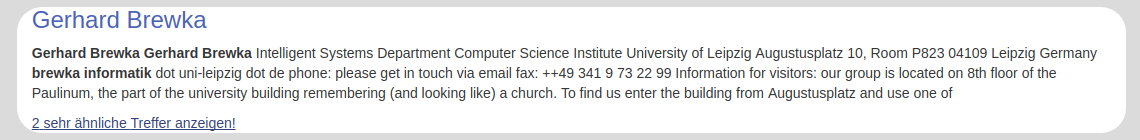
\includegraphics[width=0.99\textwidth]{chapter_data_aqcuisition/grouped_duplicates.png}
	\caption{Ein Dokument mit 2 Fast-Duplikaten}
	\label{fig:grouped_sim}
\end{figure}

\begin{wrapfigure}{H}{0.51\linewidth}
	\vspace*{-0.4cm}

\begin{scriptsize}
\begin{algorithm}[H]
	\SetKwInOut{Input}{Input}
	\SetKwInOut{Output}{Output}
		       
	\Input{ Document $\mathcal{D}$, $min$ $\in$ $\mathbb{N}^{+}$, $\mathcal{Q}$ $\in$ $\mathbb{R}$}
	\Output{ Fingerprint for Document $\mathcal{D}$}

	$\mathcal{D}$ $\gets$ removeNonAlphanumericCharacters($\mathcal{D}$)\\
	$\mathcal{D}$ $\gets$ toLowerCase($\mathcal{D}$)\\
	$\mathcal{T}$ $\gets$ tokenizeWithFrequencyCount($\mathcal{D}$)\\
	$\mathcal{T}$ $\gets$ removeTokensShorterOrEqualThan($min$, $\mathcal{T}$)\\
	$\mathcal{T}$ $\gets$ roundFreqeunciesDownToNearestMultiple($\mathcal{Q}$, $\mathcal{T}$)\\
	$\mathcal{T}$ $\gets$ removeTokensWithTooSmallFrequency($\mathcal{Q}$, $\mathcal{T}$)\\

	return md5Hash(sort($\mathcal{T}$))\\
	\caption{Text Profile}
	\label{alg:text_profile}
\end{algorithm}
\end{scriptsize}

	\vspace*{-0.2cm}
\end{wrapfigure}


Um dies zu ermöglichen, müssen zuerst die (Fast-)Duplikate identifiziert werden.
Dafür wurde das
\href{https://github.com/apache/nutch/blob/master/src/java/org/apache/nutch/crawl/TextProfileSignature.java}{TextProfileSignature}-Verfahren verwendet.
Dieser Algorithmus weist einem Dokument einen Fingerprint zu.
Dabei werden ähnliche Dokumenten auf den gleichen Wert abgebildet.
Algorithmus~\ref{alg:text_profile} zeigt dies im Pseudocode.
In Beispiel~\ref{example:text_profile} wird der Fingerprint für einen Text berechnet.

Nach der Zuweisung des Fingerprints werden entsprechend dem Discovery Scenario alle Paare von Fast-Duplikaten
gesucht~\cite{croft.chap3}. Durch dieses Vorgehen entstehen Gruppen ähnlicher Dokumente.
Für jede solche Gruppe wird ein Repräsentant gewählt\footnote{Das längste Dokument wird der Vertreter.}.
Dieser wird um die URLs der anderen Gruppenmitglieder angereichert.
Abschließend werden die restlichen Dokumente einer Gruppe gelöscht\footnote{Die Implementierung ist in dem Modul 
\href{https://github.com/mam10eks/search-homepage-of-university-leipzig/tree/master/custom-index-cleaning}
{Custom Index Cleaning} zu finden.}.

\newpage
\begin{example}[Berechnung des Fingerprints mittels TextProfileSignature]{example:text_profile}
	\textbf{Eingabe:}\\
		$\mathcal{D}$ $=$ \glqq Tropical fish include fish found in tropical environments around the world,
			including both freshwater and salt water species.\grqq,
		MINLENGTH $=$ $2$, QuantRate $=$ $0.01$\\
	
	\textbf{Tokenisierung und Filterung nach Wortlänge:}\\
		$\{$ (include, 1), (including, 1), (salt, 1), (environments, 1), (around, 1), (water, 1),
			(both, 1), (tropical, 2), (the, 1), (found, 1), (world, 1), (species, 1), (and, 1), (fish, 2), (freshwater, 1) $\}$\\

	\textbf{Filtere Einträge, deren Quantity unter Threshold liegt:}\\
		textProfile $=$ $\{$ (tropical, 2), (fish, 2) $\}$\\
	
	\textbf{Berechne Signatur:}\\
		sort(textProfile)\\
		textProfileSignature $=$ md5Hash(textProfile)
\end{example}



\newpage
\section{Verarbeitung von Anfragen}
\label{chap:query_processing}

Die Verarbeitung von Anfragen\footnote{Auch Query Processing} wird im Allgemeinen durch drei Komponenten realisiert~\cite{croft.chap2}.
Auch die im Rahmen dieser Arbeit erstellte Suchmaschine bildet davon keine Ausnahme.
Dementsprechend werden in den folgenden Abschnitten die Bestandteile User Interaction, Ranking und Evaluation vorgestellt.

\subsection{User Interaction~\cite{croft.chap2}}
\label{chap:user_interaction}

Die Komponente zur Nutzerinteraktion bietet eine Schnittstelle\footnote{Der Quellcode ist in dem Modul
\href{https://github.com/mam10eks/search-homepage-of-university-leipzig/tree/master/search-engine-backend}{search-engine-backend}
enthalten.}
zwischen dem Benutzer und der Suchmaschine.
Um diesem Nutzer eine gewohnte Usability inklusive intuitiver Bedienung zu ermöglichen,
wurden die in der Praxis verbreiteten Standards eingehalten.

\begin{wrapfigure}{H}{0.49\linewidth}
	\vspace*{-0.4cm}
	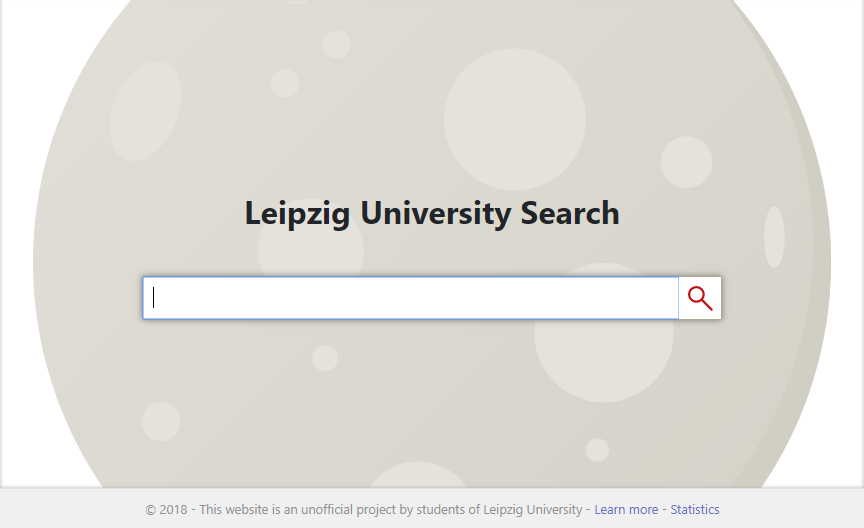
\includegraphics[width=0.48\textwidth]{chapter_query_processing/frontend_landing_page.png}
	\caption{Die Landing Page der Suchmaschine}
	\label{fig:landing_page}
	\vspace*{-0.2cm}
\end{wrapfigure}


Dementsprechend muss einem Nutzer das Absenden von Anfragen ermöglicht werden.
Dafür ist es üblich, eine Landing Page mit prominent mittig platzierter Eingabemaske auszuliefern\cite{baeza_yates.search_interfaces}.
Abbildung~\ref{fig:landing_page} zeigt dies für die im Rahmen dieser Arbeit entwickelte Suchmaschine.

Nachdem ein Nutzer seine Anfrage spezifiziert hat, werden ihm die Ergebnisse präsentiert.
Dafür erhält die Schnittstelle eine für die Query gerankte Liste von Dokumenten von der Ranking-Komponente.
Diesbezüglich ist es gängig, einem Benutzer für kleinere Ausschnitte aus der Dokumentliste jeweils 
ausgewählte Metadaten in Verbindung mit einem 
für die Anfrage besonders relevanten Textausschnitt\footnote{Sogenannte Snippets} zu präsentieren~\cite{baeza_yates.search_interfaces}.
Relevante Wörter werden dabei speziell hervorgehoben.
Die unter Berücksichtigung dieser Punkte entstandene Search Engine Result Page\footnote{SERP} wird in Abbildung~\ref{fig:serp} vorgestellt.

\begin{figure}[!ht]
	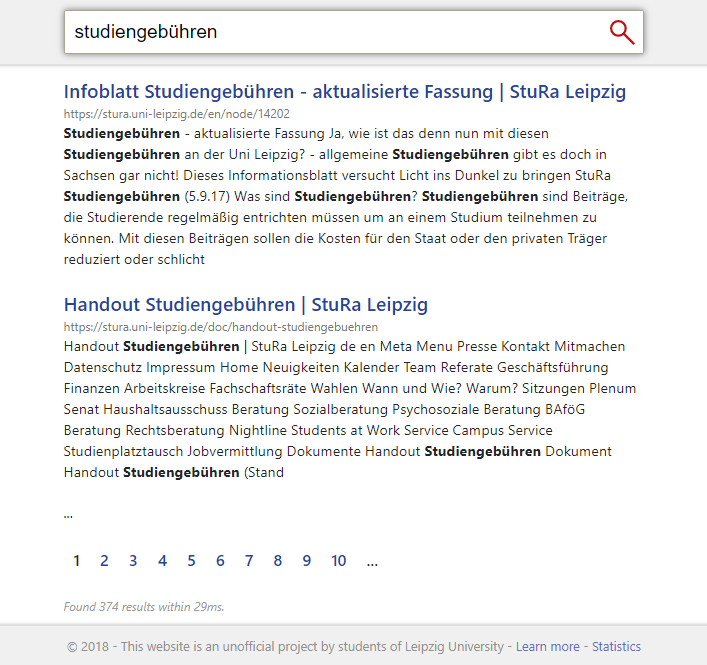
\includegraphics[width=0.99\textwidth]{chapter_query_processing/serp.png}
	\caption{Die SERP für die Anfrage \glqq studiengebühren\grqq}
	\label{fig:serp}
\end{figure}

In der Regel wird einem Nutzer die Formulierung und Spezialisierung seiner Anfragen durch verschiedene Hilfsmittel
erleichtert.
In dem vorliegenden Projekt wurde eine Query Suggestion implementiert,
welche Vervollständigungsvorschläge auf Basis populärer Anfragen liefert.
Die dafür notwendige, dynamische Benutzerschnittstelle wird in Abbildung~\ref{fig:query_suggestions} gezeigt.
Verwandte Maßnahmen zur Verbesserungen der Benutzbarkeit wie Spell Checking oder Query Refinement 
wurden zugunsten anderer Features nicht umgesetzt.

\begin{figure}[!ht]
	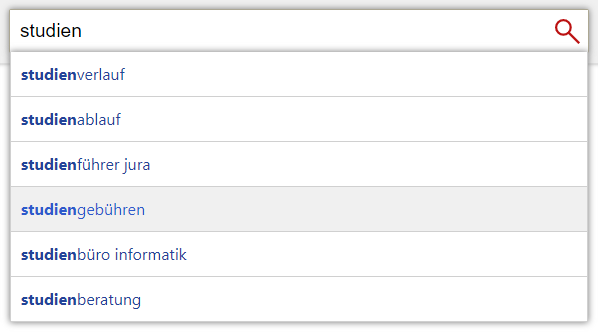
\includegraphics[width=0.99\textwidth]{chapter_query_processing/autocomplete.png}
	\caption{Query Suggestions für die Eingabe: studien}
	\label{fig:query_suggestions}
\end{figure}

Um den Suchmaschinenservice einem möglichst breiten Nutzerkreis zuzuführen, sind die
Komponenten zur Benutzerinteraktion in Form eines Webfrontends realisiert. Für die Entwicklung
werden die jeweils aktuellen Standards HTML5, CSS3 sowie JavaScript eingesetzt. 
Ausgeliefert werden diese Bestandteile durch einen Express-Webserver, welcher im Rahmen einer NodeJS-Anwendung betrieben wird.
Aus Kompatibilitätsgründen werden Teile der Bootstrap-Library eingebunden.
Falls ein Browser die History-API unterstützt, wird diese zur
Bereitstellung von Deep-Links ohne einen Full-Page-Refresh
geeigneter Seiten\footnote{Zum Beispiel die About-Page.} verwendet.

Der Zugriff auf die Ranking-Komponente (siehe Abschnitt~\ref{chap:ranking}) und Query-Suggestions wird durch
entsprechende \href{https://en.wikipedia.org/wiki/Representational_state_transfer}{REST-Endpunkte} ermöglicht.
Bereitgestellt werden diese durch eine \href{https://projects.spring.io/spring-boot/}{Spring-Boot-Anwendung}.
Die Query-Suggestions unterscheiden dabei zwischen nutzerbezogenen und globalen Vorschlägen.
Durch nutzerbezogene Vorschläge ist es einem Nutzer möglich, von ihm bereits getätigte Anfragen zu wiederholen.
Globale Vorschläge identifizieren innerhalb der Suchmaschine populäre Anfragen mit Hilfe von Logdaten.
Für eine sinnvolle initiale Menge von globalen Vorschlägen wurden semantisch passende
Vorschläge von Google gecrawlt und eingepflegt\footnote{Der Quellcode für den Crawler ist TODO link zum Code.
Damit wurden 2639 Vorschläge generiert}.


\subsection{Ranking~\cite{croft.chap2}}
\label{chap:ranking}
Die Ranking-Komponente ist der Kern jeder Suchmaschine.
Sie erzeugt für eine Query aus der User-Interaction-Komponente eine gerankte Liste von Dokumenten.

Dabei beeinflussen deren Effizienz\footnote{Die Verarbeitung vieler Anfragen in kurzer Zeit.}
und Effektivität\footnote{Die Qualität des Rankings: Kann die Suchmaschine relevante Informationen finden?}
die Nützlichkeit der Suchmaschine wesentlich.
Um für beide Anforderungen einen sinnvollen Ausgangspunkt zu schaffen, wurde für das Ranking
\href{https://lucene.apache.org/}{Lucene} verwendet.
Diese Software stellt einen geeigneten Einstieg dar, da darauf andere,
in dieser Domäne verbreitete Softwarekomponenten aufbauen\footnote{Insbesondere die verbreiteten Tools~\cite{dbengines}
\href{https://de.wikipedia.org/wiki/Elasticsearch}{Elasticsearch} und \href{http://lucene.apache.org/solr/}{Solr}
basieren auf Lucene. Deren erweiterter Funktionsumfang, wie Beispielsweiße eine
\href{http://www.searchdatacenter.de/definition/Horizontale-Skalierung-Scale-out}{horizontale Skalierung}, wurde im Rahmen dieser Arbeit nicht benötigt.}.
Verschiedene \href{https://en.wikipedia.org/wiki/Ranking_(information_retrieval)}{Ranking-Algorithmen}
\footnote{Und damit auch 
\href{https://de.wikipedia.org/wiki/Information_Retrieval\#Retrievalmodelle}{Retrieval-Modelle}}
sind in Lucene verfügbar.

Davon wurde \href{https://en.wikipedia.org/wiki/Okapi_BM25}{BM25F} eingesetzt,
da es als Baseline für modernere Ranking-Algorithmen fungiert und für allgemeine
Dokumentsammlungen bessere Ergebnisse\footnote{Entsprechendes Tuning der von BM25F verwendeten Parameter vorrausgesetzt~\cite{baeza_yates.107}.}
erzielt als die verfügbaren,
\href{https://opensourceconnections.com/blog/2015/10/16/bm25-the-next-generation-of-lucene-relevation/}{klassischen Vektor-Modelle}~\cite{baeza_yates.107}.
Dieses \href{https://de.wikipedia.org/wiki/Information_Retrieval#Retrievalmodelle}{Retrieval-Modell}
besitzt die Fähigkeit, mehrere Felder\footnote{Felder werden auch als Attribute oder Features bezeichnet.} in die Berechnung des Scores einfließen zu lassen.
Entsprechend wurden alle verfügbaren Felder 
einbezogen\footnote{Alle Felder mit unmittelbarem Bezug zu dem Inhalt der Dokumente.
Dies sind der vollständige Text eines Dokuments, sowie deren Titel, URL und Anchor-Texte eingehender Links.}.
Da eine sinnvolle Wahl der Attribute\footnote{Einschließlich eventuell abgeleiteter Features.}
und deren Gewichtung im Allgemeinen in
Verbindung mit der User-Relevanz steht, wurden alle Parameter bei ihren Standards belassen.

Das entsprechende Vorgehen für ein Tuning basierend auf Nutzer-Feedback
wird in Abschnitt~\ref{chap:log_analysis} vorgestellt.



\subsection{Evaluation~\cite{croft.chap2}}
\label{chap:evaluation}
Die Aufgabe der Evaluationskomponente ist es, Effizienz und Effektivität zu monitoren.
Dafür muss eine Aufzeichnung des Nutzerverhaltens sowie ausgewählter Systemmetriken vorgenommen werden.

Insbesondere zur Aufzeichnung des Nutzerverhaltens ist eine Identifikation der Nutzer notwendig.
Darauf aufbauend kann protokolliert werden, welcher Nutzer welche Anfragen ausgeführt
hat, welche Ergebnisseiten oder Query-Suggestions einem Nutzer präsentiert wurden,
sowie gegebenenfalls welche Ergebnisse oder Query Suggestions ausgewählt
wurden\footnote{Das erweitern dieser Informationen um die entsprechenden Event-Zeitpunkte erlaubt eine
sinnvolle Rekonstruktion des Nutzerverhaltens.}.

Bei einer technischen Realisierung dieser Punkte fällt auf,
dass es sich um sogenannte \href{https://de.wikipedia.org/wiki/Cross-Cutting_Concern}{Cross-Cutting Concerns}
handelt. Ein bewährtes Mittel derartige Funktionalitäten zu realisieren, ohne die
Komplexität der betroffenen Systemteile unnötig zu ehöhen,
stellt die Aspektorientierte Programmierung\footnote{AOP} dar\cite{spring.chap1.1}.
Die darin verwendeten Aspekte definieren,
was\footnote{In der zugehörigen AOP Terminologie definiert der zu einem Aspekt gehörende Advice die Aufgabe,
also was von dem Aspekt zu erledigen ist~\cite{spring.chap4.1}.}, wann\footnote{Der Advice eines Aspekts definiert 
neben dem was auch zu welchen Zeitpunkten ein Aspekt auszuführen ist.
Unter anderem kann vor, nach, oder das wrappen einer Zielmethode spezifiziert werden\cite{spring.chap4.1}.}
und wo\footnote{Durch sogenannte Pointcuts werden eine oder mehrere Methoden definiert,
an die der Advice gewoben wird\cite{spring.chap4.1}.} auszuführen ist\cite{spring.chap4.1}.

In dem für die Interaction-Komponente verwendeten Framework werden alle Endpunkte über speziell anotierte Methoden
bereitgestellt.
Diesen ist gemein, dass sie ein
\href{https://de.wikipedia.org/wiki/Plain_Old_Java_Object}{POJO}\footnote{Diese sind 
entsprechend einer gewählten Konvention in dem 
\href{https://github.com/mam10eks/search-homepage-of-university-leipzig/tree/master/search-engine-backend}{Backend-Modul}
in zugehörigen \href{https://de.wikipedia.org/wiki/Transferobjekt}{dto} Paketen definiert.}
als Model für die Antwort zurückgeben. 
Dieses Modell wird je nach Endpunkt später in ein HTML-Template\footnote{Spezifiziert innerhalb des 
\href{https://github.com/mam10eks/search-homepage-of-university-leipzig/tree/master/search-engine-backend/src/main/resources/templates}
{templates-Ordner in dem Backend-Modul}.} gerendert oder
JSON-serialisiert.

Unter diesen Vorraussetzungen eignen sich diese Methoden hervorragend,
um sie durch Aspekte um die gewünschten Funktionalitäten zu erweitern\footnote{Schließlich lassen
sie sich eindeutig und generisch über die notwendigen Endpunkt-Anotationen
identifizieren.}.
Dazu wird ein Effizienz-, ein User-Identification-, sowie ein Logging-Aspekt eingesetzt.
Der Effizienz-Aspekt misst dabei Beispielhaft für weitere Systemmetriken die Bearbeitungszeit von Anfragen,
und erweitert das zurückgegebene Model entsprechend.
Der User-Identification-Aspekt stellt
vor dem Aufruf jeder Endpunkt-Methode sicher, dass der Request mit einer
eindeutigen Identifikation des Nutzers versehen ist.
Dies wird über einen Cookie realisiert.
Der Logging-Aspekt protokolliert ausnahmslos alle verfügbaren Informationen.
Dazu notiert er für jeden Endpunkt den Request des Clients zusammen mit dem zurückzugebenden
POJO-Model\footnote{Mit diesem Vorgehen lassen sich alle angesprochenen Informationen zur Rekonstruktion des Nutzer-Verhaltens erheben,
da insbesondere die Links zu den Dokumenten auf dem Server durch Weiterleitungen aufgelöst werden.}.

Die vom Logging-Aspekt protokollierten Informationen können sowohl
Online\footnote{Beispielhaft wurde das im Rahmen dieser Arbeit für die Query-Suggestions vorgenommen.},
als auch Offline analysiert werden.
Um beides zu ermöglichen, wurde mit \href{https://kafka.apache.org/}{Apache Kafka}
eine Streaming Platform mit der Möglichkeit zur persistenten Datenhaltung~\cite{kafka.foreword} eingesetzt.
Dazu publisht der Logging-Aspekt seine Daten als Events nach Kafka.
Um diesen Logging-Aspekt so einfach wie möglich zu halten, bereitet ein
\href{https://www.confluent.io/blog/introducing-kafka-streams-stream-processing-made-simple/}{Stream Processor}
diese Daten weiter auf\footnote{Dieser Stream Processor reichert die Events an und leitet sie
auf sinnvolle Topics um. Der Quellcode ist in dem Modul 
\href{https://github.com/mam10eks/search-homepage-of-university-leipzig/tree/master/search-engine-kafka-streams}
{search-engine-kafka-streams} enthalten.}.
Online-Analysen wie die Query-Suggestion können sich nun unmittelbar an die für sie interessanten Events subscriben.
Offline Analysen können die persistierten Events gleichzeitig in einem  Batch-Vorgang verarbeiten.
Als Beispiel dafür stellt Abbildung~\ref{fig:visualization} einen mit Python realisierten
Import\footnote{Der Quellcode ist in dem Modul
\href{https://github.com/mam10eks/search-homepage-of-university-leipzig/tree/master/visualize_events}{visualize\_events}.}
der Events nach \href{https://de.wikipedia.org/wiki/Neo4j}{Neo4j} zur Visualisierung dar.

\begin{figure}[!ht]
	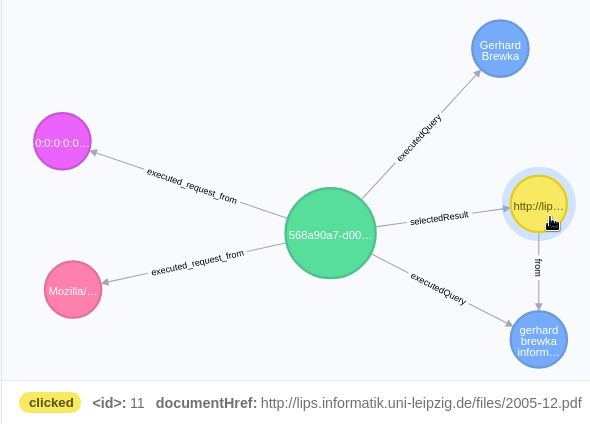
\includegraphics[width=0.99\textwidth]{chapter_query_processing/example_neo4j_visualization.png}
	\caption{Beispielgraph im
	\href{https://neo4j.com/developer/guide-neo4j-browser/}{Neo4j-Browser}
	einer User-Session bestehend aus 2 Anfragen, bei denen bei einer Anfrage ein Ergebniss angeklickt wurde.}
	\label{fig:visualization}
\end{figure}

Die hier vorgestellte Evaluationskomponente funktioniert für alle Clients, welche Cookies erlauben und den \href{}{Referrer-Header}
korrekt setzen.



\newpage
\section{Analyse der Logdaten}
\label{chap:log_analysis}

Bla

\subsection{Durchführung eines Laborexperiments}
\label{chap:labroratory_experiment}

Bla


%************************************************************************************************************************
%* bibliography
%************************************************************************************************************************
\newpage
\addcontentsline{toc}{section}{Literatur}
\bibliography{literature}
\bibliographystyle{alpha}

\end{document}
